\section{Casi d'uso}
L'analisi del capitolato, gli incontri con l'azienda \AZIENDA\ e la discussione tra gli \textit{Analisti} interni al gruppo Stark Labs hanno portato alla definizione dei casi d'uso a seguire. Ogni caso d'uso è identificato da un codice univoco gerarchico, nella forma:\\
\begin{center}
UC[codice univoco del padre].[codice progressivo di livello]
\end{center}
Il codice progressivo può includere diversi livelli di profondità separati da un punto.

\subsection{Caso d'uso UC1: Scenario di alto livello}
\label{sec:UC1}

\begin{itemize}
\item \textbf{Attore}: utente;
\item \textbf{Scopo e descrizione}: l'utente ha avviato correttamente l'applicazione per creare sceneggiati. L'applicazione è ora pronta all'uso. Possono essere effettuate diverse operazioni: l'utente può creare un nuovo sceneggiato oppure modificarne uno già avviato. Inoltre l'utente può salvare il suo lavoro, esportarlo in formato audio o video e opzionalmente condividerlo;
\item \textbf{Precondizione}: il programma è avviato e pronto all'uso;
\item \textbf{Flusso principale degli eventi}:
\begin{enumerate}
\item L'utente può creare un nuovo sceneggiato o lavorare su un progetto già iniziato (UC1.1, UC1.8);
\item L'utente può esportare lo sceneggiato sotto forma di video o audio (UC1.4, UC1.3);
\item L'utente può salvare lo sceneggiato (UC1.6);
\item L'utente può condividere il file audio o il video dello sceneggiato (UC1.2).
\end{enumerate}
\item \textbf{Estensioni}: in caso di errori durante la fase di condivisione l'applicazione si occuperà di esportare lo sceneggiato in un file audio o video da salvare nel sistema;
\item \textbf{Postcondizione}: l'applicazione ha ottenuto le informazioni sulle operazioni che l'utente desidera eseguire.
\end{itemize}

\begin{figure}[H]
\centering
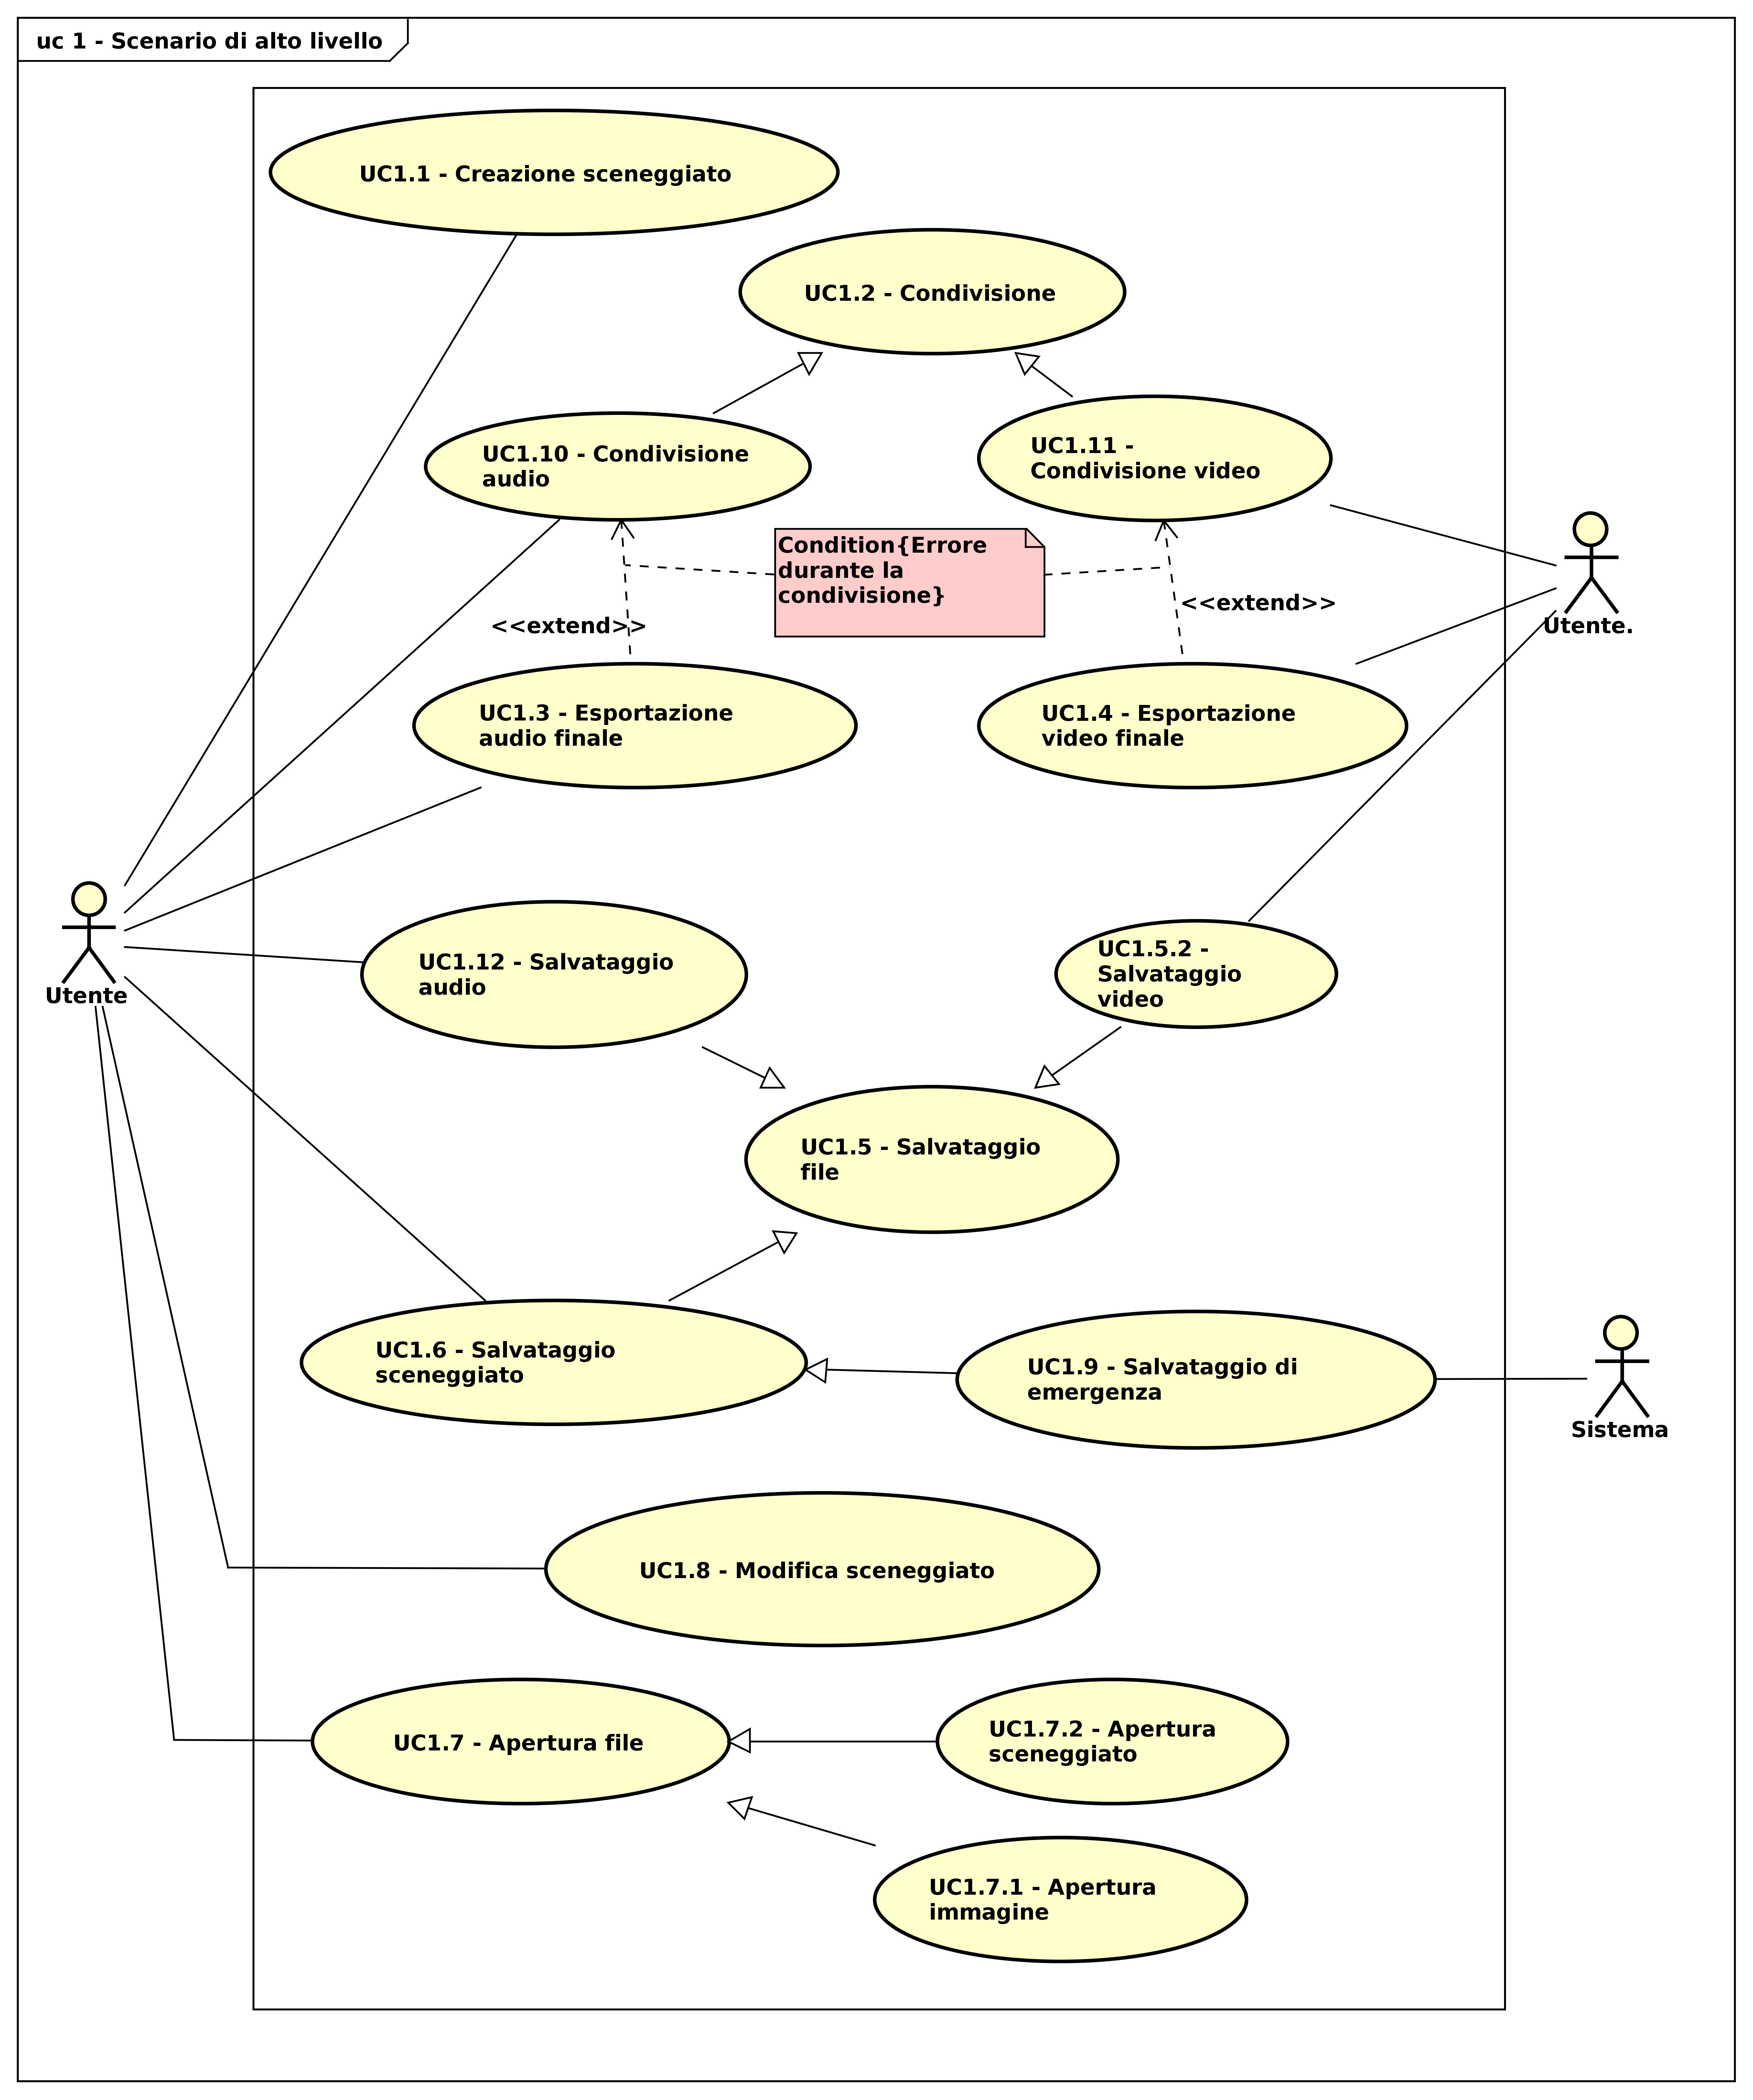
\includegraphics[scale=0.5]{immagini/uc1_scenario_alto_livello.png}
\captionsetup{labelfont=bf}
\caption{Caso d'uso UC1}
\end{figure}
\newpage


\subsection{Caso d'uso UC1.1: Creazione sceneggiato}
\label{sec:UC1.1}


\begin{itemize}
\item \textbf{Attore}: utente;
\item \textbf{Scopo e descrizione}: l'utente ha scelto di creare un nuovo sceneggiato. L'utente deve poter inserire i capitoli che lo costituiscono, caratterizzare i personaggi che vi fanno parte e poter scrivere le battute;
\item \textbf{Precondizione}: il sistema è pronto a creare un nuovo sceneggiato;
\item \textbf{Flusso principale degli eventi}:
\begin{enumerate}
\item L'utente può assegnare un titolo allo sceneggiato (UC1.1.6);
\item L'utente può creare un nuovo personaggio dello sceneggiato (UC1.1.1);
\item L'utente può modificare o cancellare un personaggio (UC1.1.7, UC1.1.8);
\item L'utente può creare un nuovo capitolo (UC1.1.2);
\item L'utente può modificare un capitolo (UC1.1.3);
\item L'utente può riordinare i capitoli alterandone la sequenza (UC1.1.4);
\item L'utente può cancellare un capitolo (UC1.1.5).
\end{enumerate}
\item \textbf{Postcondizione}: l'applicazione ha creato un nuovo sceneggiato.
\end{itemize}

\begin{figure}[htbp]
\centering
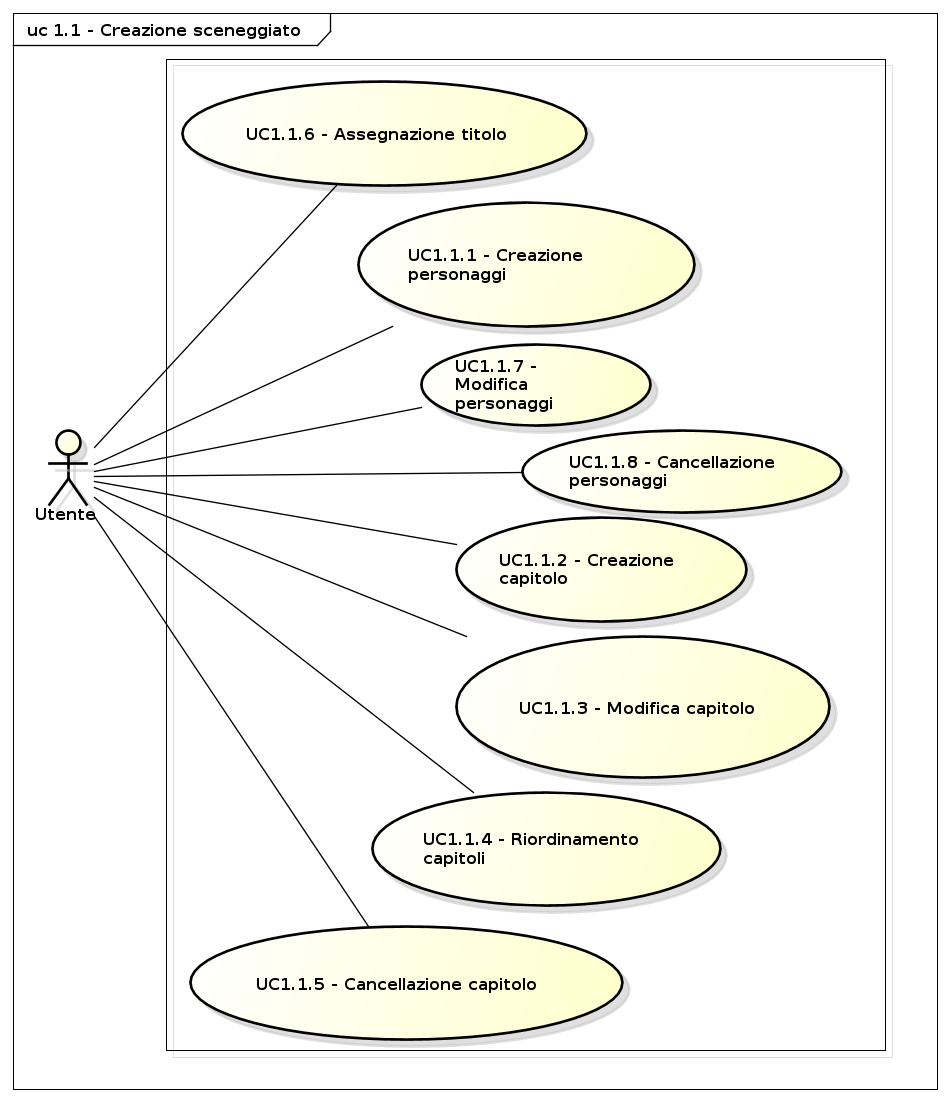
\includegraphics[scale=0.5]{immagini/uc1_1_creazione_sceneggiato.png}
\captionsetup{labelfont=bf}
\caption{Caso d'uso UC1.1}
\end{figure}
\newpage

\subsection{Caso d'uso UC1.1.1: Creazione personaggi}
\label{sec:UC1.1.1}

\begin{itemize}
\item \textbf{Attore}: utente;
\item \textbf{Scopo e descrizione}: l'utente può creare un nuovo personaggio per il suo sceneggiato associandoci nome, \textit{avatar\G} e voce;
\item \textbf{Precondizione}: il sistema è pronto a creare un nuovo personaggio;
\item \textbf{Flusso principale degli eventi}:
\begin{enumerate}
\item L'utente assegna un nome al nuovo personaggio (UC1.1.1.1);
\item L'utente assegna un \textit{avatar} al nuovo personaggio, ossia l'immagine con cui il personaggio viene raffigurato nello sceneggiato (UC1.1.1.3);
\item L'utente assegna una voce (\textit{preset}\G) al nuovo personaggio (UC1.1.1.2);
\item L'utente può creare una nuova voce, che in seguito può essere assegnata al personaggio (UC1.1.1.4);
\item L'utente può modificare una voce già esistente, prima di assegnarla al personaggio (UC1.1.1.5).
\end{enumerate} 
\item \textbf{Scenari alternativi}: se il server di \AZIENDA\ non è raggiungibile, è possibile assegnare al personaggio una voce predefinita di sistema;
\item \textbf{Postcondizione}: il sistema crea un nuovo personaggio.
\end{itemize}

\begin{figure}[htbp]
\centering
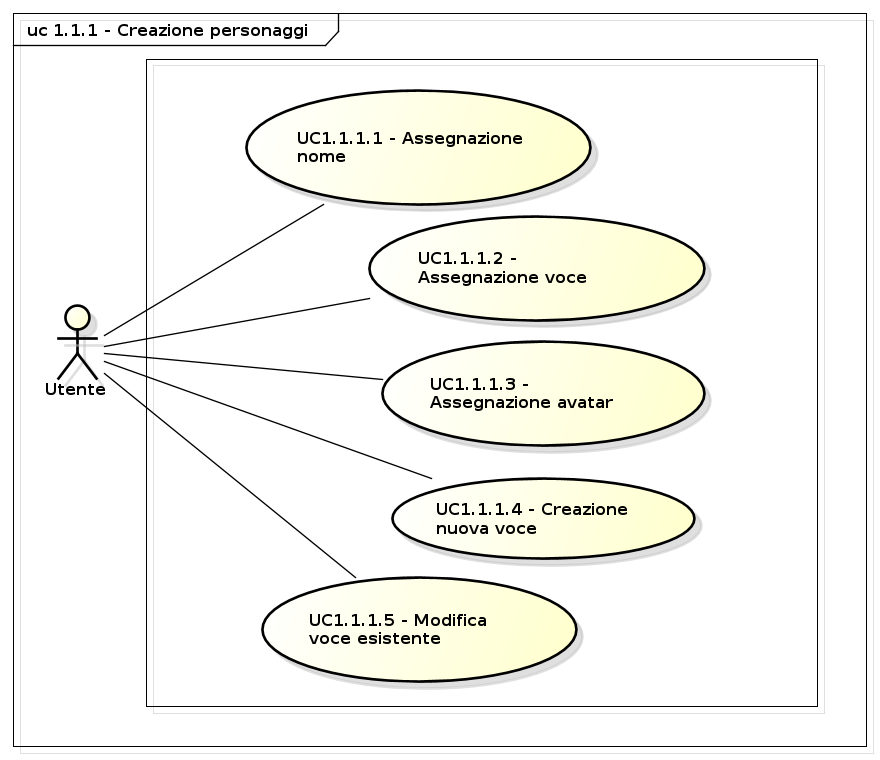
\includegraphics[scale=0.5]{immagini/uc1_1_1_creazione_personaggi.png}
\captionsetup{labelfont=bf}
\caption{Caso d'uso UC1.1.1}
\end{figure}
\newpage

\subsection{Caso d'uso UC1.1.1.2: Assegnazione voce}
\label{sec:UC1.1.1.2}
\begin{itemize}
\item \textbf{Attore}: utente;
\item \textbf{Scopo e descrizione}: l'utente assegna a un personaggio una fra le voci disponibili; 
\item \textbf{Precondizione}: il sistema è pronto a ricevere la selezione di una voce;
\item \textbf{Flusso principale degli eventi}:
\begin{enumerate}
\item L'utente può navigare tra le voci disponibili (UC1.1.1.2.1);
\item L'utente seleziona una voce (UC1.1.1.2.2).
\end{enumerate}
\item \textbf{Postcondizione}: il sistema associa la voce selezionata al personaggio.
\end{itemize}

\subsection{Caso d'uso UC1.1.1.4: Creazione nuova voce}
\label{sec:UC1.1.1.4}

\begin{itemize}
\item \textbf{Attore}: utente;
\item \textbf{Scopo e descrizione}: l'utente può creare un nuova voce che può essere in seguito associata a un personaggio. La creazione di una voce avviene mediante la configurazione di un insieme di effetti e parametri;
\item \textbf{Precondizione}: il sistema è pronto a creare una nuova voce e ha caricato i parametri richiesti;
\item \textbf{Flusso principale degli eventi}:
\begin{enumerate}
\item L'utente seleziona una lingua (UC1.1.1.4.1);
\item L'utente seleziona il sesso della voce (UC1.1.1.4.2);
\item L'utente può modificare i parametri degli effetti applicabili (UC1.1.1.4.3);
\item L'utente può assegnare un nome alla voce (UC1.1.1.4.4).
\end{enumerate} 
\item \textbf{Scenari alternativi}: nel caso in cui il server di \AZIENDA\ non fosse raggiungibile, verranno rese disponibili le sole voci di sistema, alle quali non è possibile applicare effetti;
\item \textbf{Postcondizione}: il sistema memorizza la nuova voce.
\end{itemize}
\begin{figure}[htbp]
\centering
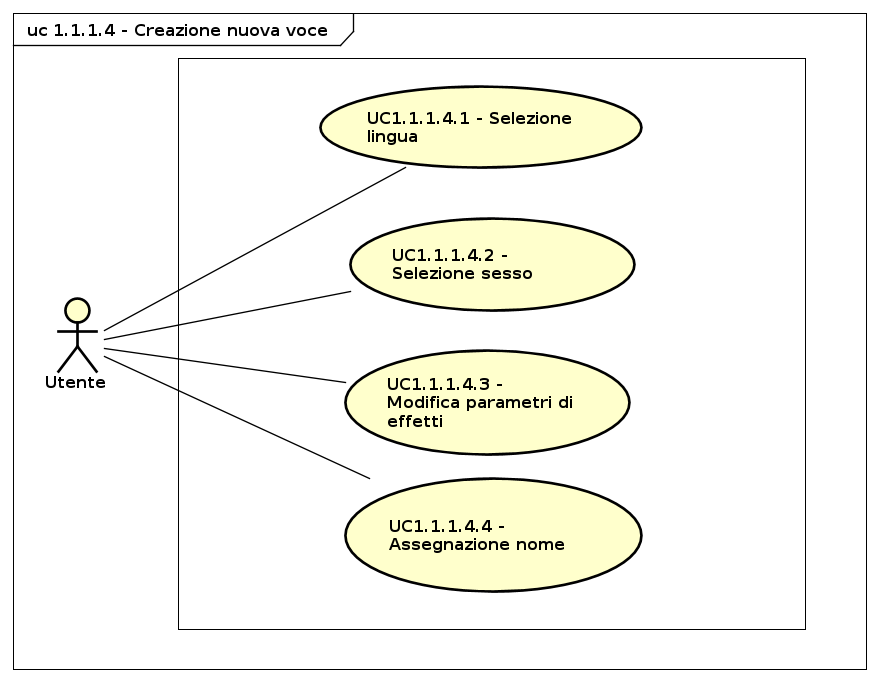
\includegraphics[scale=0.5]{immagini/uc1_1_1_4_creazione_nuova_voce.png}
\captionsetup{labelfont=bf}
\caption{Caso d'uso UC1.1.1.4}
\end{figure}
\newpage

\subsection{Caso d'uso UC1.1.2: Creazione capitolo}
\label{sec:UC1.1.2}

\begin{itemize}
\item \textbf{Attore}: utente;
\item \textbf{Scopo e descrizione}: l'utente può creare un capitolo dello sceneggiato. Nello specifico può inserire un'immagine di sfondo alla scena e scrivere le battute che i personaggi si scambiano in questo contesto. Ad ogni battuta possono essere applicati degli effetti, alcuni dei quali possono suggerire una determinata emozione;
\item \textbf{Precondizione}: l'utente ha creato uno sceneggiato e ci ha associato dei personaggi;
\item \textbf{Flusso principale degli eventi}:
\begin{enumerate}
\item L'utente assegna un titolo al capitolo (UC1.1.2.1);
\item L'utente crea lo sfondo, ossia il contesto visivo e sonoro in cui i personaggi si scambiano le battute (UC1.1.2.2);
\item L'utente scrive una nuova battuta (UC1.1.2.3);
\item L'utente può modificare una battuta (UC1.1.2.4);
\item L'utente può cancellare una battuta (UC1.1.2.5);
\item L'utente può associare alle battute degli effetti, che ne alterano il modo in cui sono sintetizzate (UC1.1.2.6);
\item L'utente può ascoltare un'anteprima del capitolo, per avere un riscontro di quanto creato in un certo momento (UC1.1.2.7);
\item L'utente può inserire un suono qualsiasi (per esempio un rumore ambientale), caricato dalla memoria o scelto fra una serie di suoni forniti (UC1.1.2.8). 
\end{enumerate} 
\item \textbf{Postcondizione}: è stato creato un capitolo dello sceneggiato;
\end{itemize}
\begin{figure}[htbp]
\centering
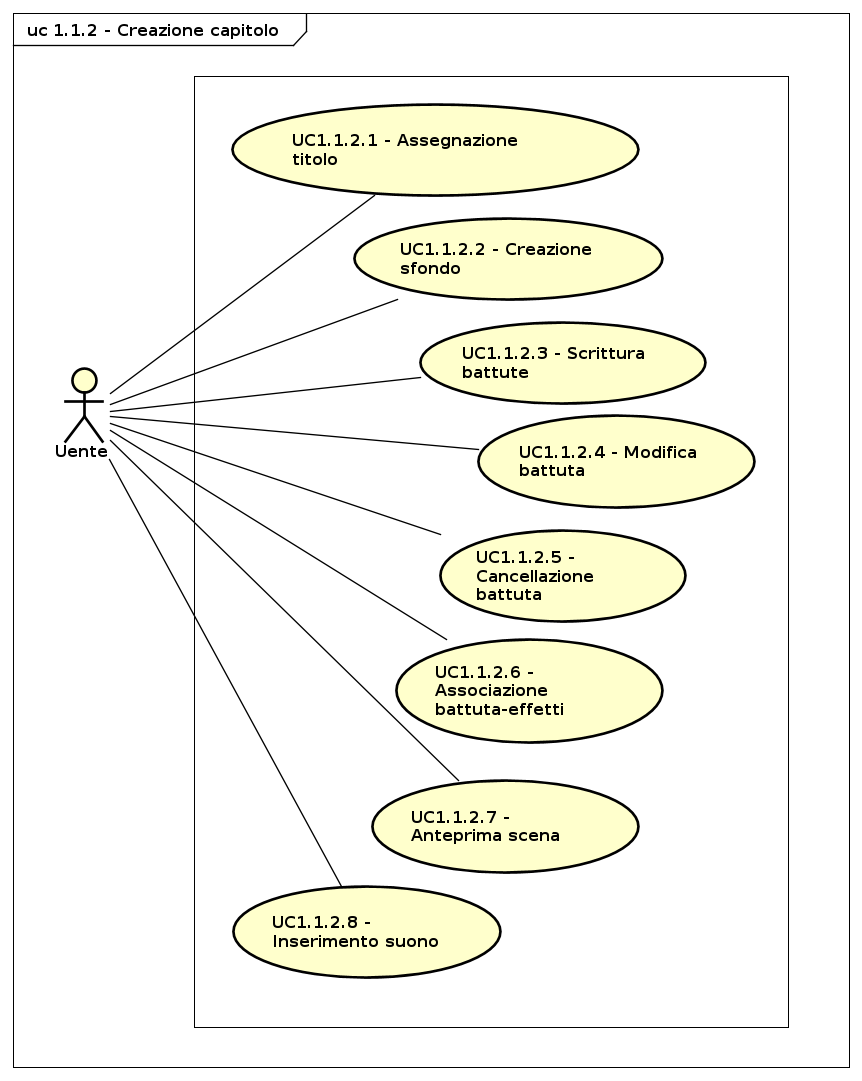
\includegraphics[scale=0.5]{immagini/uc1_1_2_creazione_capitolo.png}
\captionsetup{labelfont=bf}
\caption{Caso d'uso UC1.1.2}
\end{figure}
\newpage

\subsection{Caso d'uso UC1.1.2.2: Creazione sfondo}
\label{sec:UC1.1.2.2}

\begin{itemize}
\item \textbf{Attore}: utente;
\item \textbf{Scopo e descrizione}: l'utente può associare un'immagine e un audio di sottofondo a un capitolo creato;
\item \textbf{Precondizione}: l'utente ha creato un capitolo;
\item \textbf{Flusso principale degli eventi}:
\begin{enumerate}
\item L'utente assegna un'immagine di sfondo al capitolo, che può essere scelta da un insieme di immagini fornite, o caricata dall'utente (UC1.1.2.2.1);
\item L'utente assegna un audio di sottofondo al capitolo, scelto fra un insieme dato a disposizione, o caricato liberamente dall'utente (UC1.1.2.2.2);
\end{enumerate} 
\item \textbf{Postcondizione}: è stato creato lo sfondo di un capitolo dello sceneggiato;
\end{itemize}
\begin{figure}[htbp]
\centering
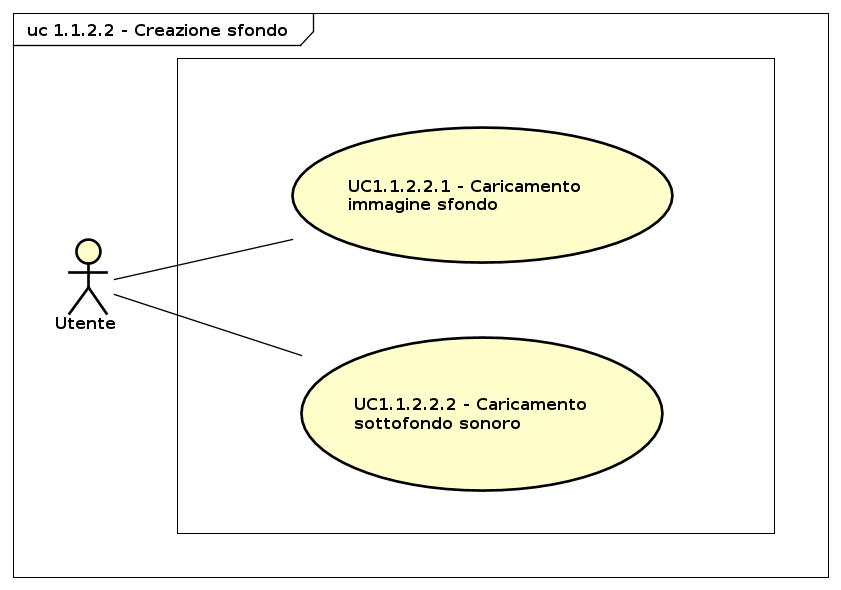
\includegraphics[scale=0.5]{immagini/uc1_1_2_2_creazione_sfondo.png}
\captionsetup{labelfont=bf}
\caption{Caso d'uso UC1.1.2.2}
\end{figure}
\newpage

\subsection{Caso d'uso UC1.1.2.3: Scrittura battute}
\label{sec:UC1.1.2.3}

\begin{itemize}
\item \textbf{Attore}: utente, modulo di sistema;
\item \textbf{Scopo e descrizione}: l'utente può digitare il testo di una nuova battuta e assegnarla a un personaggio tra quelli creati; il modulo di sistema provvede a convertire il testo inserito in SSML\G\ e a inviarlo al server di \AZIENDA; 
\item \textbf{Precondizione}: il sistema è pronto a ricevere il testo per la creazione di una nuova battuta;
\item \textbf{Flusso principale degli eventi}:
\begin{enumerate}
\item L'utente naviga tra i personaggi disponibili (UC1.1.2.3.1);
\item L'utente seleziona il personaggio a cui associare la battuta (UC1.1.2.3.2);
\item L'utente scrive il testo della nuova battuta (UC1.1.2.3.3);
\item Il modulo di sistema converte il testo della battuta scritta dall'utente in SSML (UC1.1.2.3.4).
\end{enumerate} 
\item \textbf{Postcondizione}: è stata creata una nuova battuta;
\end{itemize}
\begin{figure}[htbp]
\centering
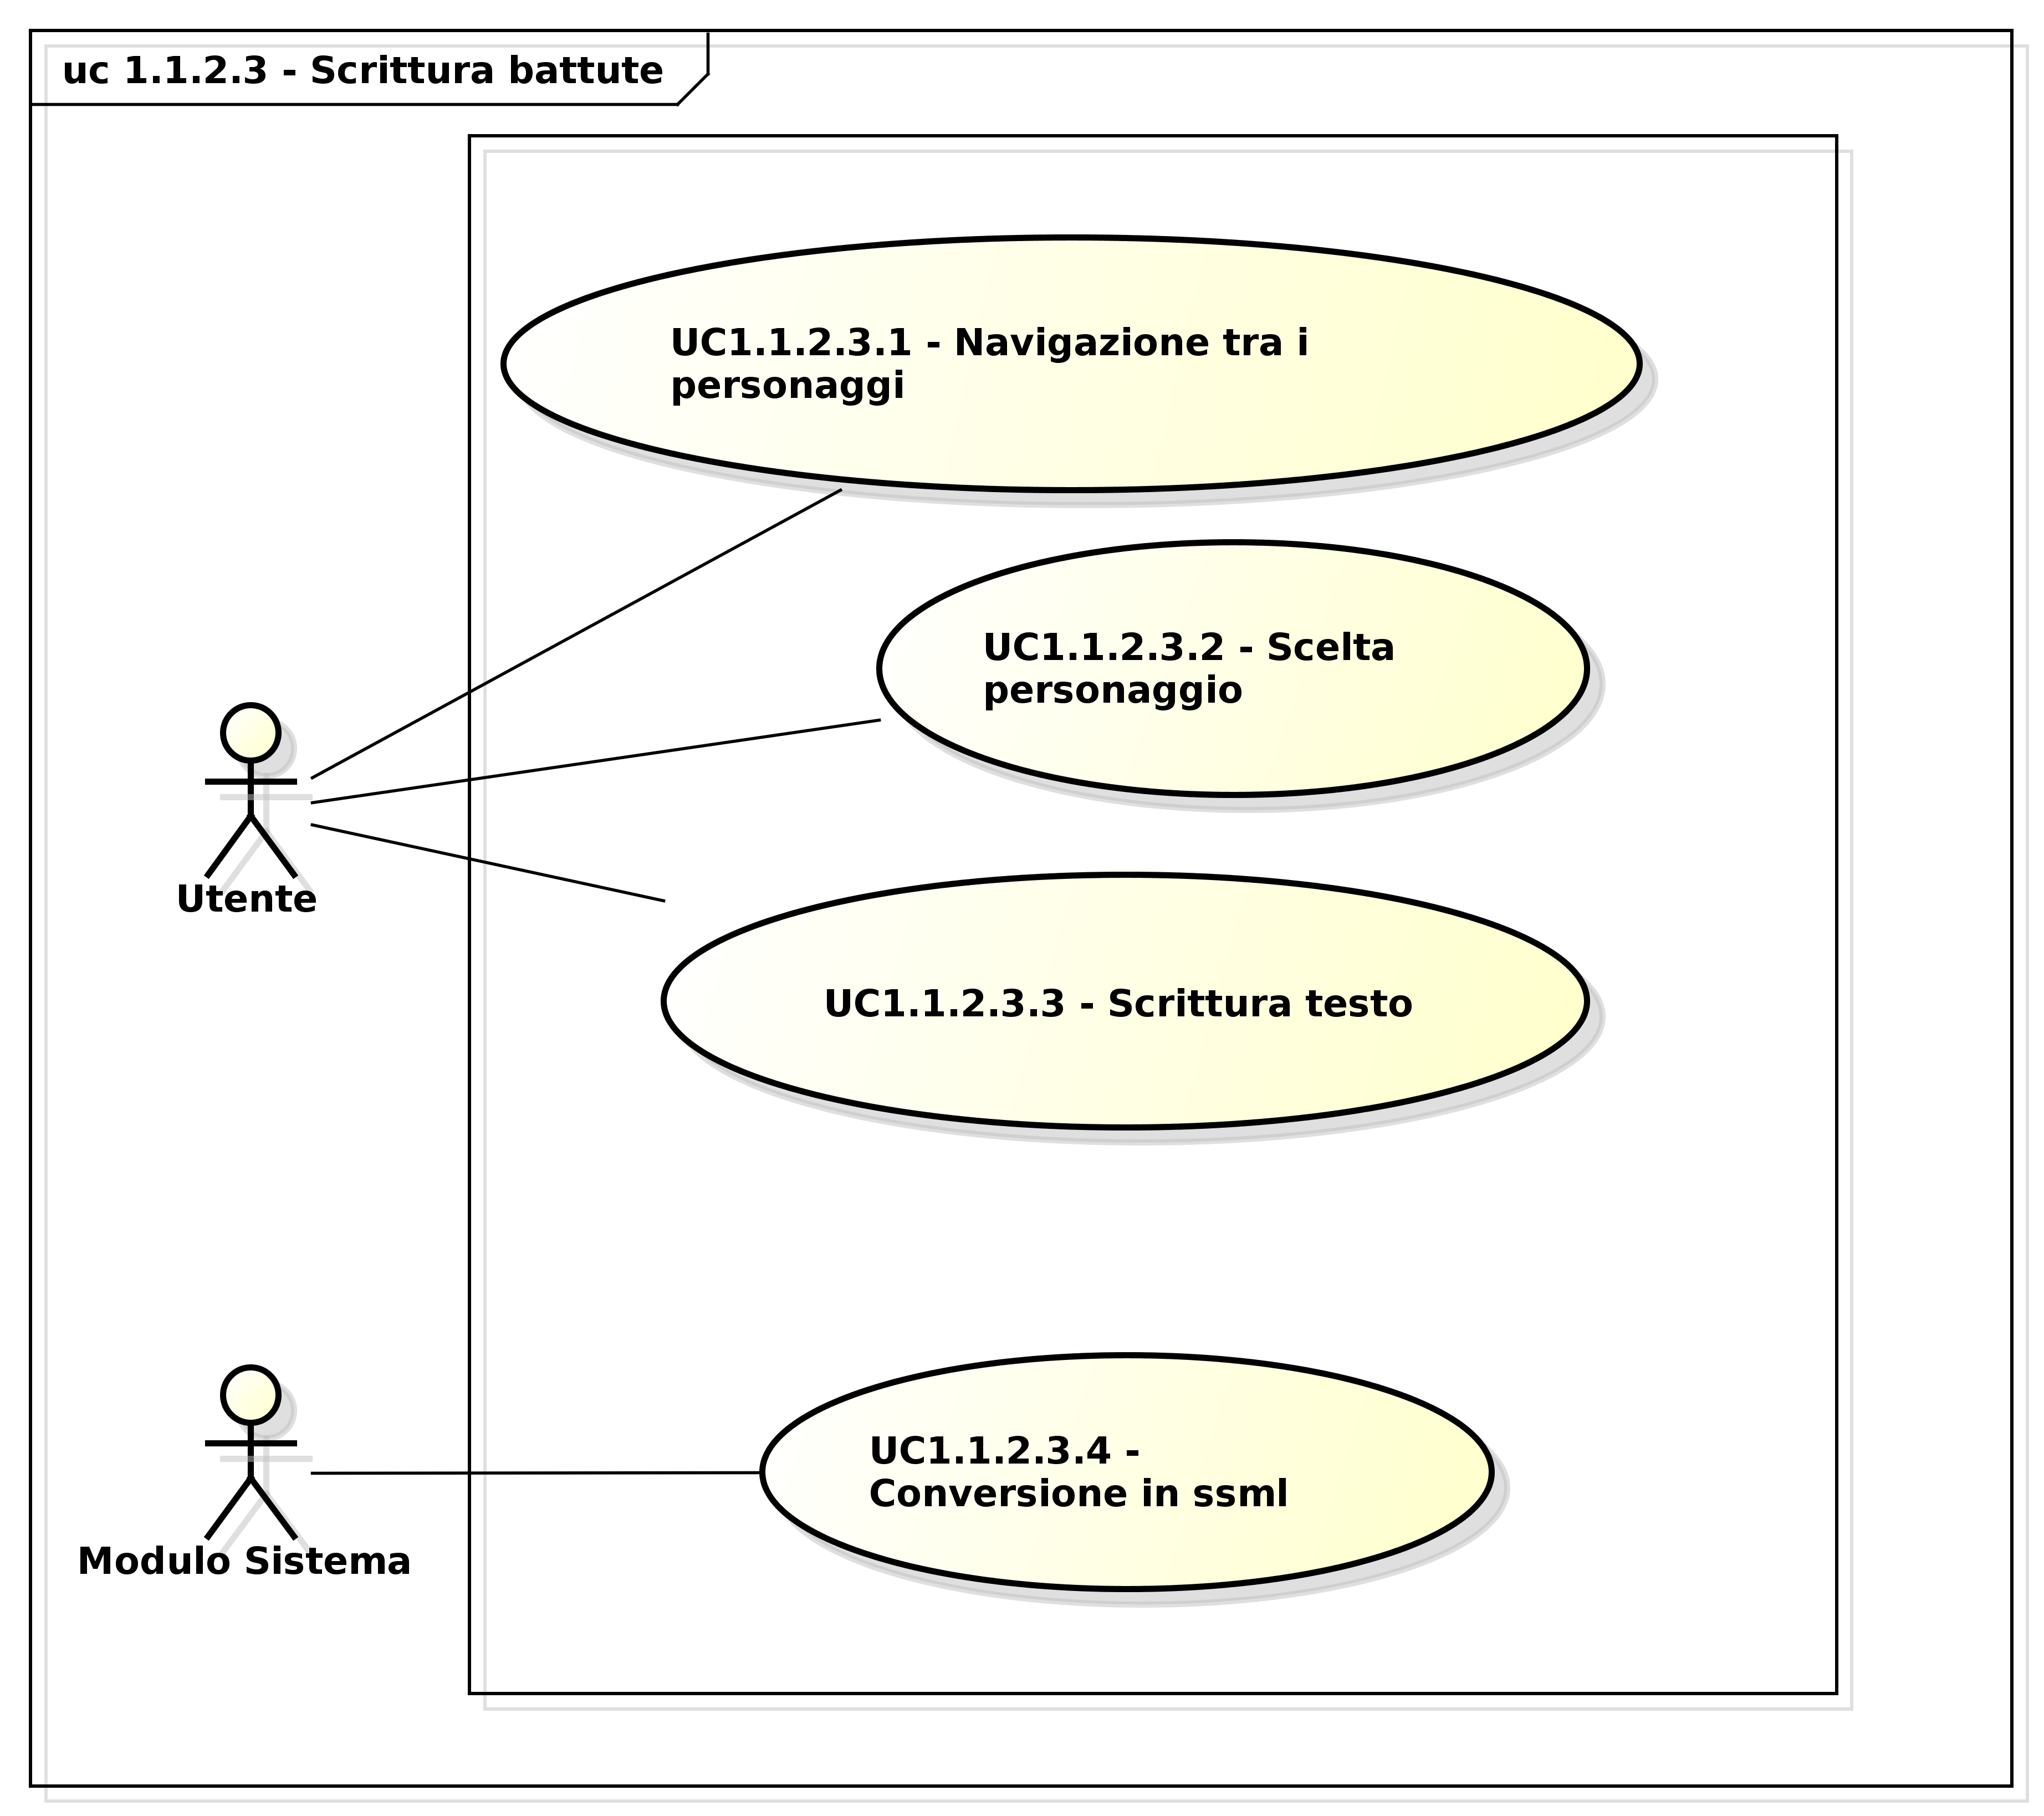
\includegraphics[scale=0.5]{immagini/uc1_1_2_3_scrittura_battute.png}
\captionsetup{labelfont=bf}
\caption{Caso d'uso UC1.1.2.3}
\end{figure}
\newpage

\subsection{Caso d'uso UC1.1.2.4: Modifica battuta}
\label{sec:UC1.1.2.4}

\begin{itemize}
\item \textbf{Attore}: utente, modulo di sistema;
\item \textbf{Scopo e descrizione}: avendo a disposizione almeno una battuta già creata, l'utente può decidere di modificarne: testo, personaggio, sentimento ed effetti associati;
\item \textbf{Precondizione}: almeno una battuta è già stata creata in precedenza;
\item \textbf{Flusso principale degli eventi}:
\begin{enumerate}
\item L'utente seleziona la battuta (UC1.1.2.4);
\item L'utente può cambiarne il testo (UC1.1.2.4.2);
\item L'utente può cambiarne il sentimento (UC1.1.2.4.3);
\item L'utente può cambiarne gli effetti associati, anche a basso livello (UC1.1.2.4.5);
\item L'utente può cambiarne il personaggio (UC1.1.2.4.4);
\item Il Modulo di Sistema converte la battuta in SSML\G\ (UC1.1.2.3.4);
\end{enumerate}
\item \textbf{Postcondizione}: è stata modificata una battuta già creata in precedenza.
\end{itemize}
\begin{figure}[htbp]
\centering
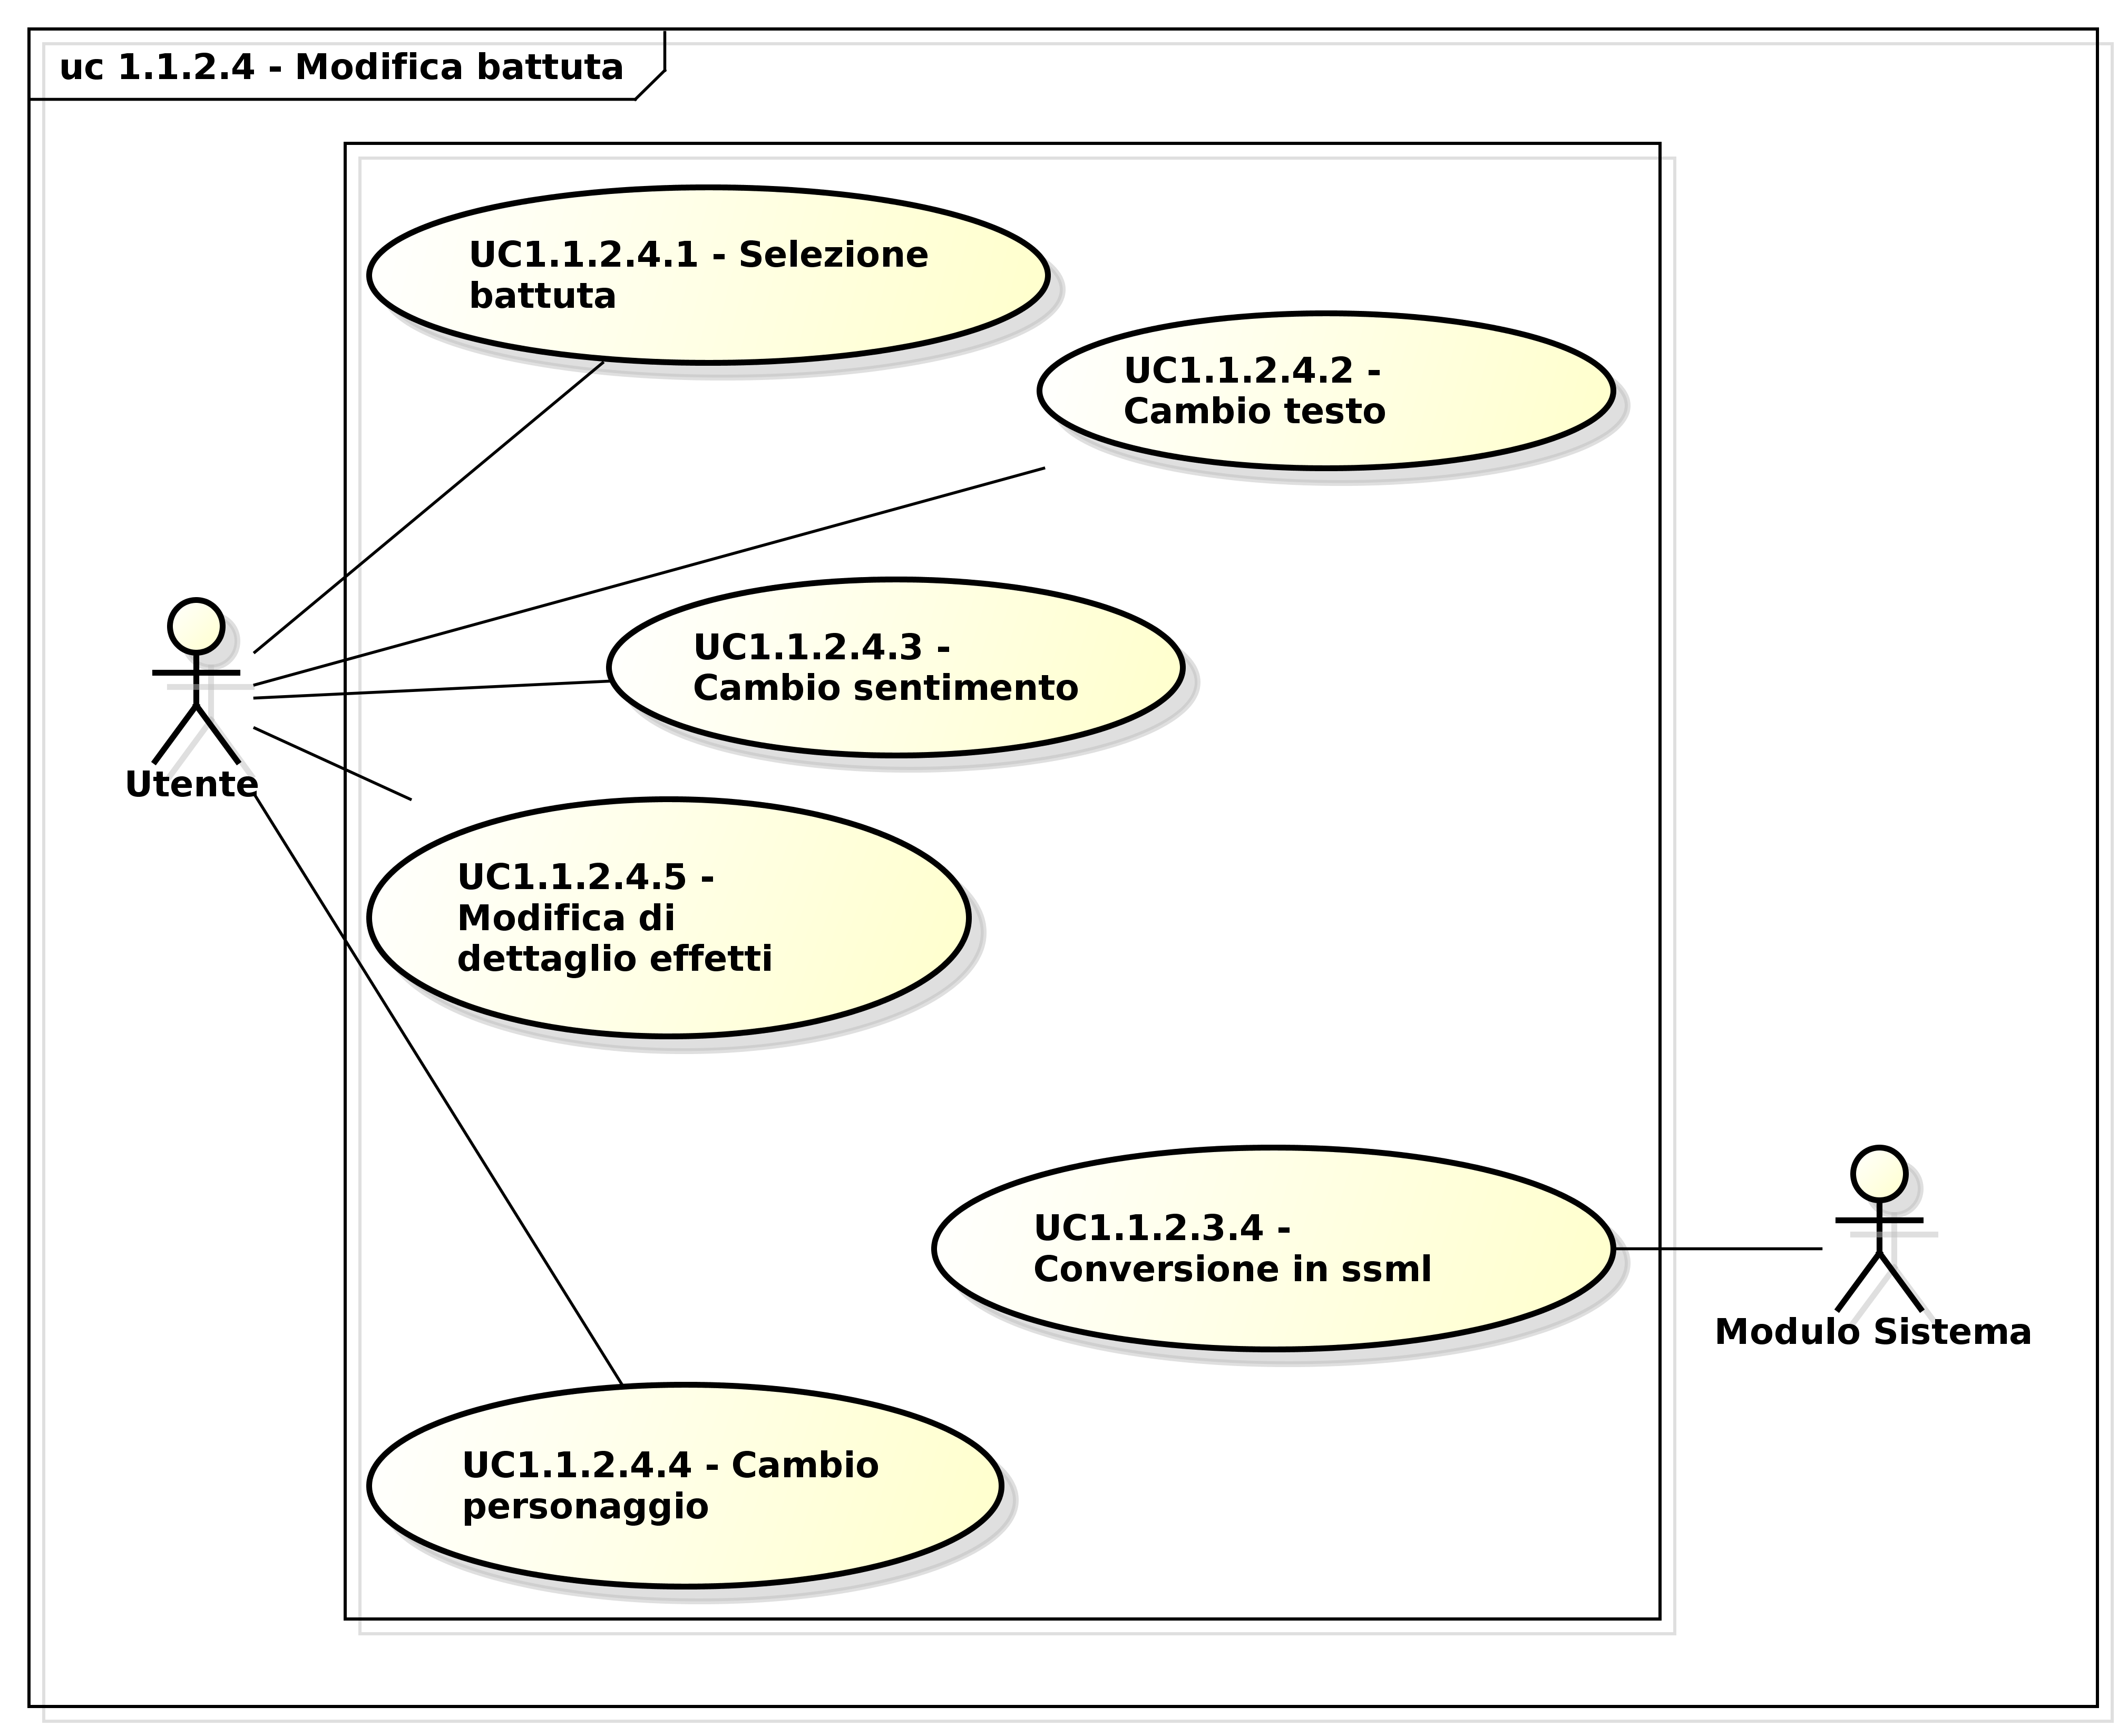
\includegraphics[scale=0.5]{immagini/uc1_1_2_4_modifica_battuta.png}
\captionsetup{labelfont=bf}
\caption{Caso d'uso UC1.1.2.4}
\end{figure}
\newpage

\subsection{Caso d'uso UC1.1.4: Associazione battuta-effetti}
\label{sec:UC1.1.4}

\begin{itemize}
\item \textbf{Attore}: utente, modulo di sistema;
\item \textbf{Scopo e descrizione}: avendo a disposizione almeno una battuta già creata, l'utente può modificare gli effetti associati e può testare le modifiche grazie a un'anteprima; 
\item \textbf{Precondizione}: almeno una battuta è già stata creata in precedenza;
\item \textbf{Flusso principale degli eventi}:
\begin{enumerate}
\item L'utente seleziona la battuta da modificare (UC1.1.2.6.1);
\item L'utente può scegliere se associare un sentimento alla battuta (UC1.1.2.6.3);
\item L'utente può scegliere di inserire delle pause nella battuta (UC1.1.2.6.4);
\item L'utente può scegliere se modificare gli effetti in dettaglio (UC1.1.2.6.5);
\item L'utente può scegliere se ascoltare un'anteprima della battuta (UC1.1.2.6.2);
\item Il Modulo di Sistema converte la battuta in SSML\G\ (UC1.1.2.6.6).
\end{enumerate}
\item \textbf{Postcondizione}: l'associazione battuta-effetti è avvenuta correttamente.
\end{itemize}
\begin{figure}[htbp]
\centering
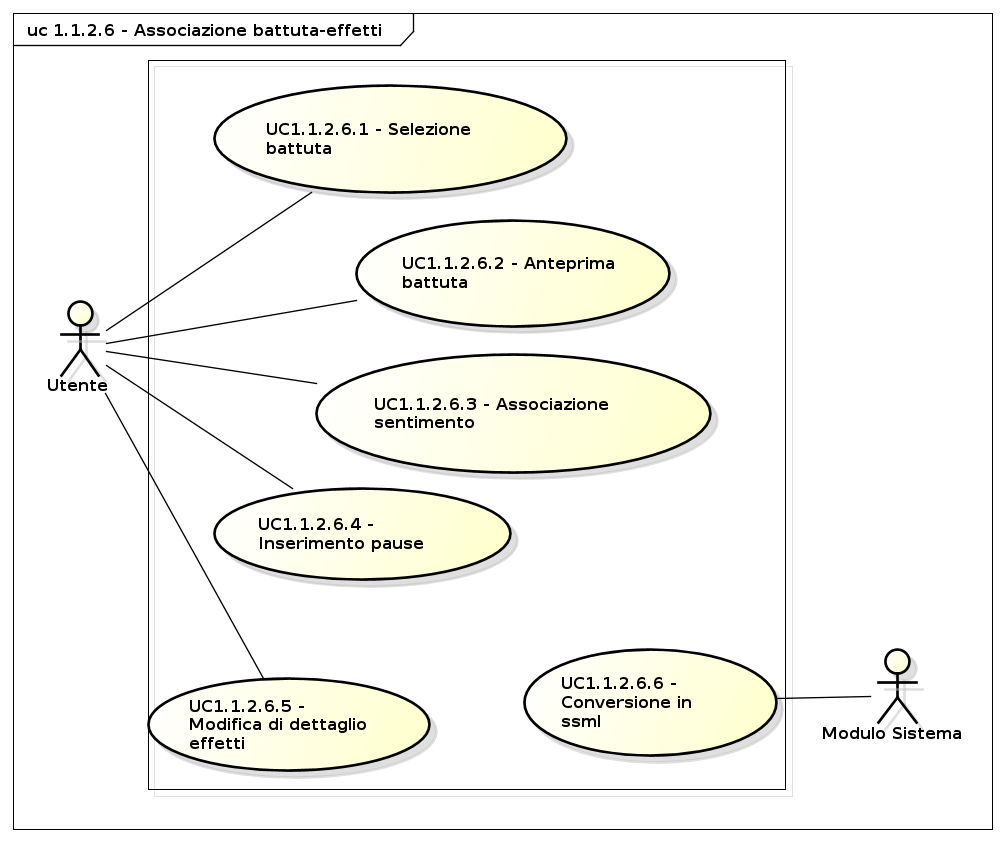
\includegraphics[scale=0.5]{immagini/uc1_1_2_6_associazione_battuta_effetti.png}
\captionsetup{labelfont=bf}
\caption{Caso d'uso UC1.1.2.6}
\end{figure}
\newpage

\subsection{Caso d'uso UC1.2: Condivisione}
\label{sec:UC1.2}

\begin{itemize}
\item \textbf{Attori}: utente, sistema;
\item \textbf{Scopo e descrizione}: l'utente può scegliere se condividere il \textit{file} relativo allo sceneggiato esportato in formato video o audio, selezionando uno tra gli strumenti di condivisione reperiti dal sistema;
\item \textbf{Precondizione}: lo sceneggiato è stato creato;
\item \textbf{Flusso principale degli eventi}:
\begin{enumerate}
\item L'utente sceglie se condividere lo sceneggiato in formato audio o video (UC1.2.4);
\item Il sistema reperisce la lista degli strumenti di condivisione presenti nel dispositivo (UC1.2.3);
\item L'utente può navigare tra gli elementi della lista sopracitata (UC1.2.1);
\item L'utente può scegliere uno tra gli elementi della lista (UC1.2.2).
\end{enumerate}
\item \textbf{Scenari alternativi}: se il dispositivo non possiede alcuno strumento di condivisione, è possibile unicamente creare un file audio o video da memorizzare nel dispositivo \textit{mobile}; 
\item \textbf{Postcondizione}: lo sceneggiato viene condiviso con successo in formato audio o video; 
\end{itemize}
\begin{figure}[htbp]
\centering
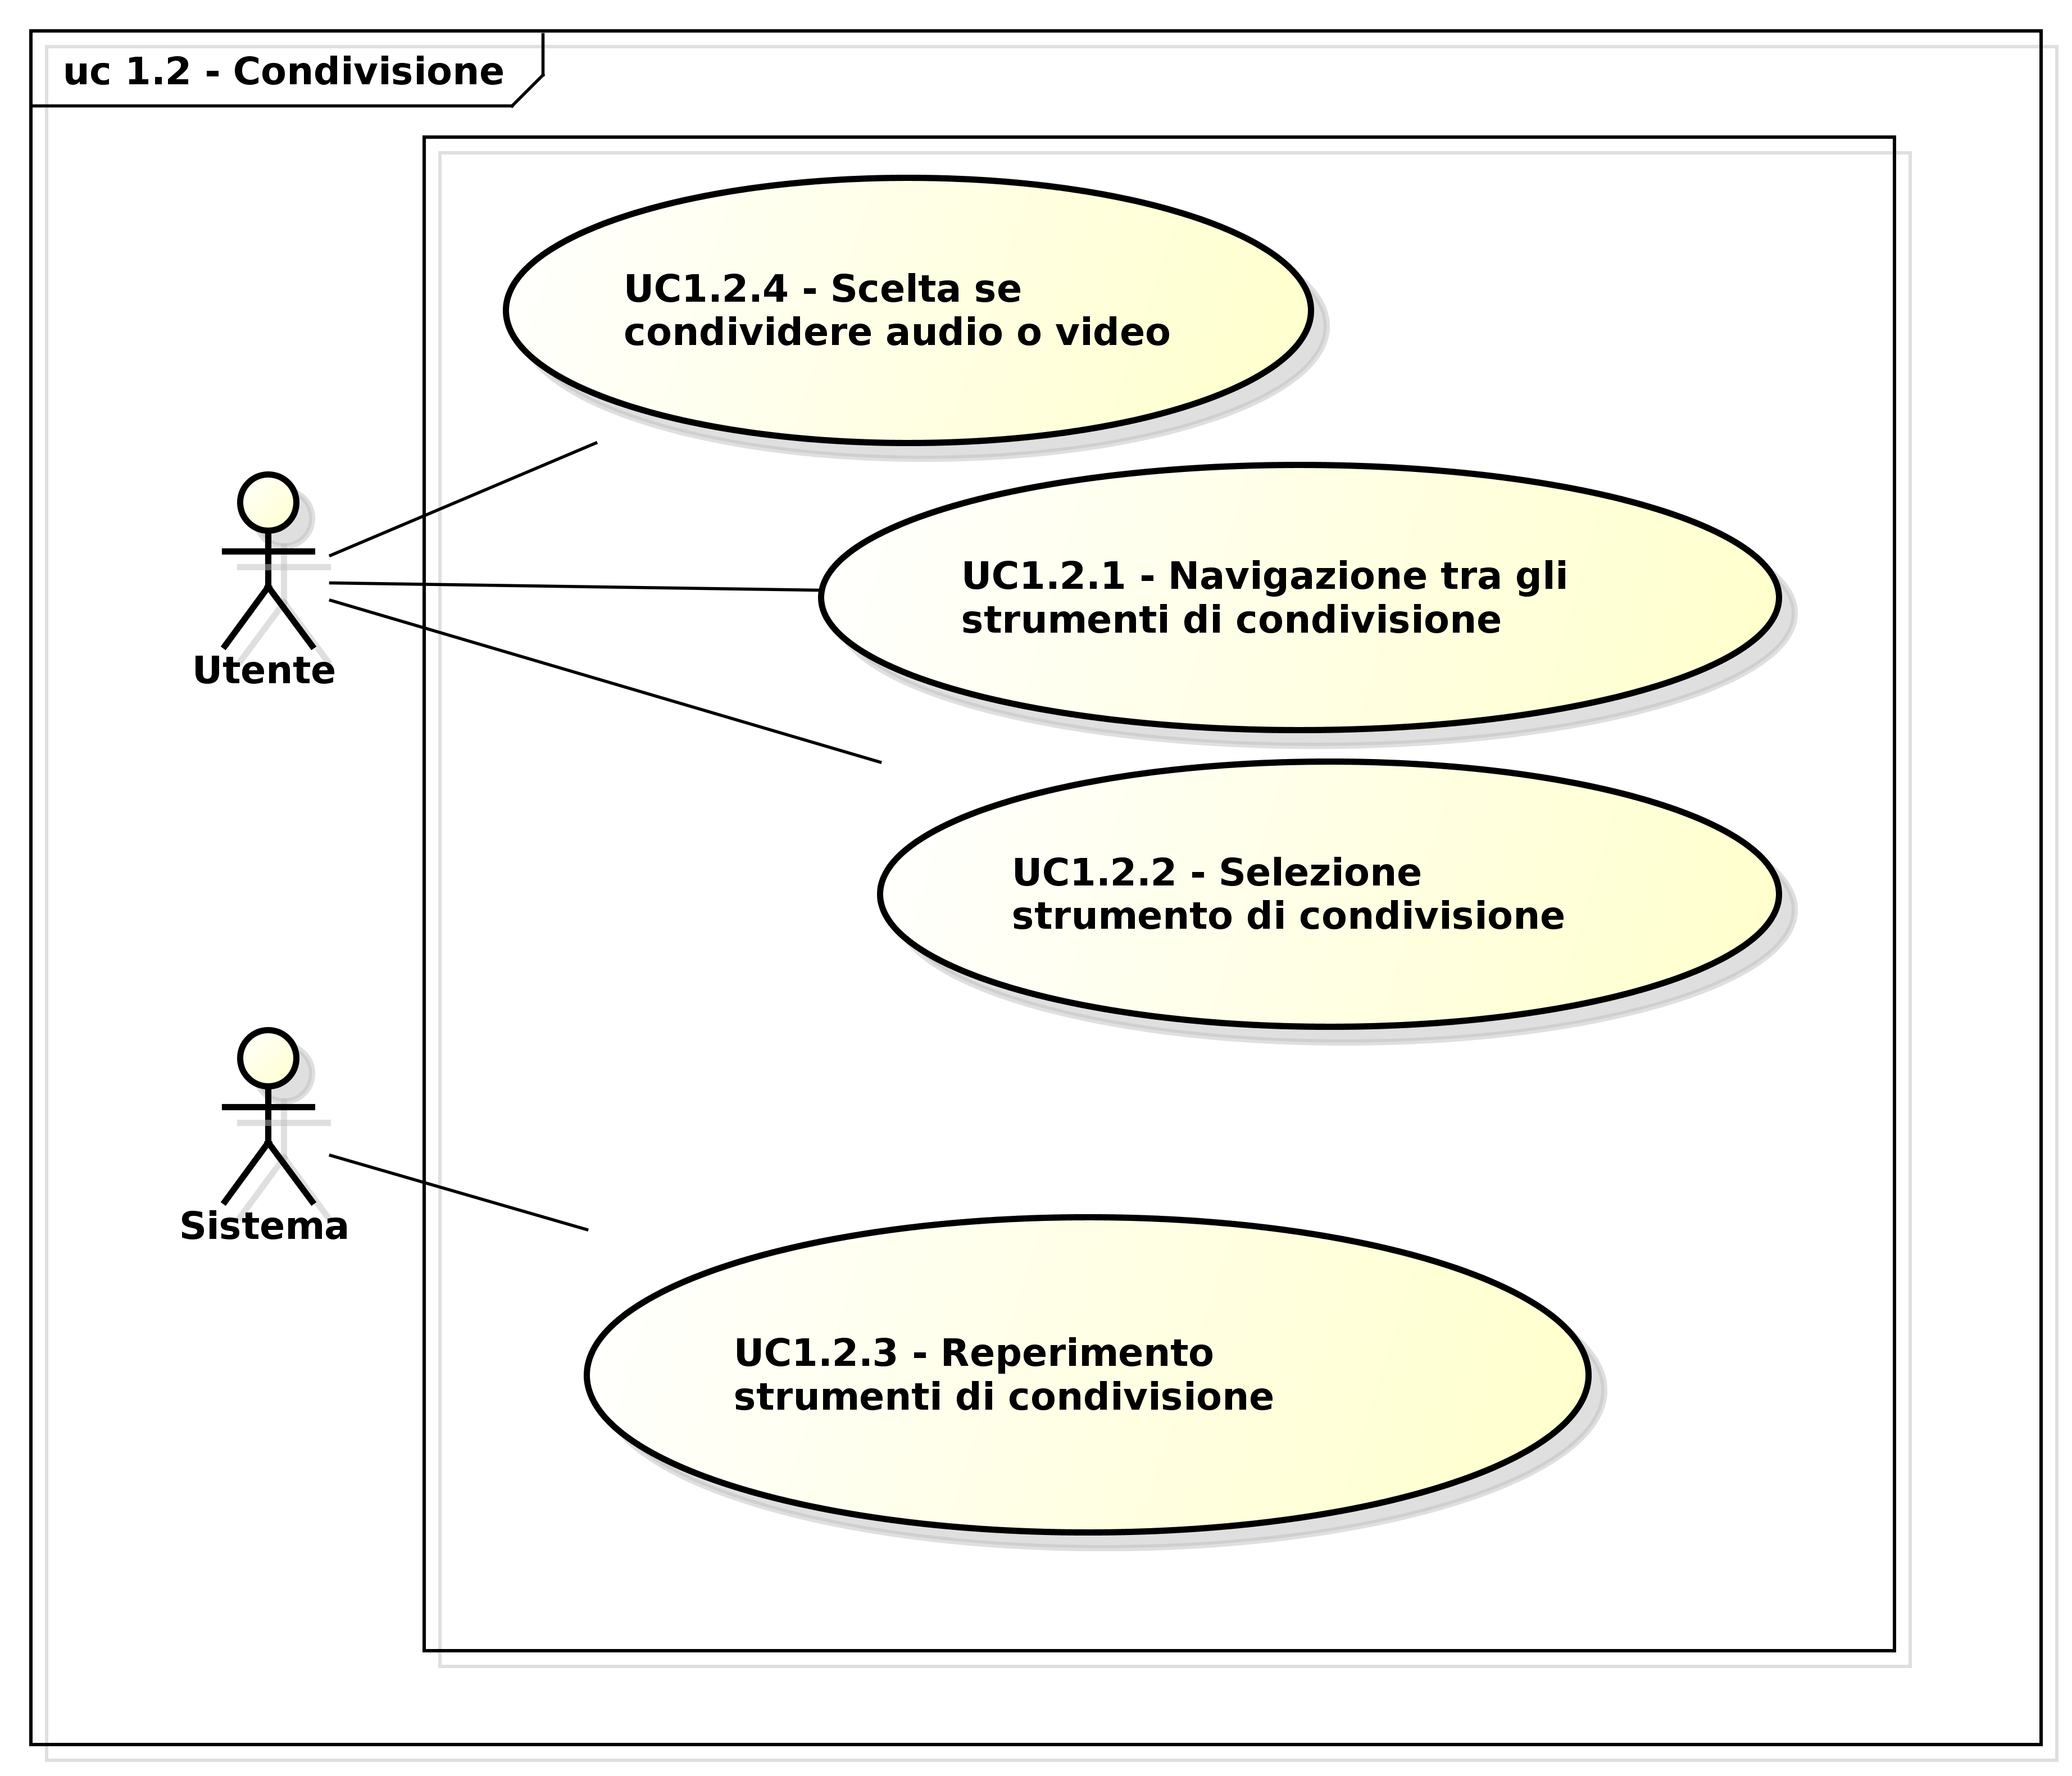
\includegraphics[scale=0.5]{immagini/uc1_2_condivisione.png}
\captionsetup{labelfont=bf}
\caption{Caso d'uso UC1.2}
\end{figure}
\newpage

\subsection{Caso d'uso UC1.3: Esportazione file audio}
\label{sec:UC1.3}

\begin{itemize}
\item \textbf{Attore}: utente;
\item \textbf{Scopo e descrizione}: l'utente può esportare lo sceneggiato in un \textit{file} audio, scegliendone il nome e il formato di esportazione;
\item \textbf{Precondizione}: il sistema è pronto a esportare uno sceneggiato correttamente formato;
\item \textbf{Flusso principale degli eventi}:
\begin{enumerate}
\item L'utente digita il nome del \textit{file} di esportazione (UC1.3.2);
\item L'utente seleziona il formato desiderato (UC1.3.1).
\end{enumerate}
\item \textbf{Postcondizione}: viene effettuata l'esportazione nel formato desiderato.  
\end{itemize}
\begin{figure}[htbp]
\centering
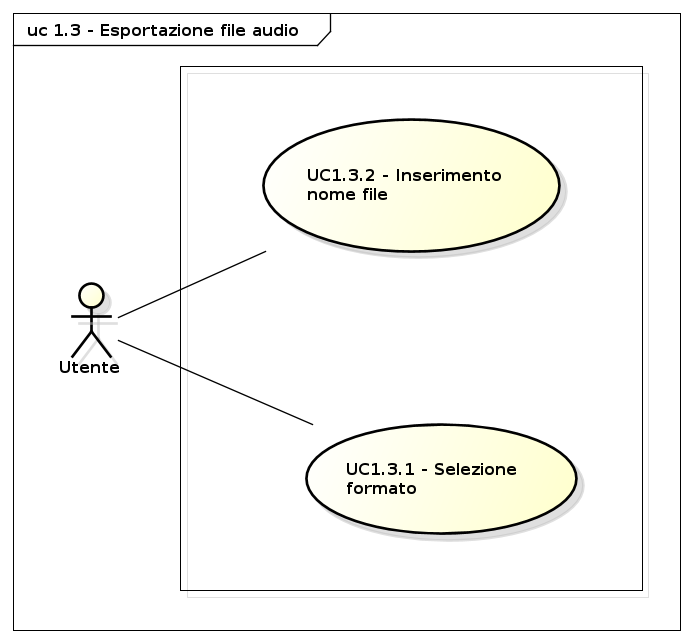
\includegraphics[scale=0.5]{immagini/uc1_3_esportazione_audio.png}
\captionsetup{labelfont=bf}
\caption{Caso d'uso UC1.3}
\end{figure}
\newpage

\subsection{Caso d'uso UC1.3: Esportazione file video}
\label{sec:UC1.3}

\begin{itemize}
\item \textbf{Attore}: utente;
\item \textbf{Scopo e descrizione}: l'utente può esportare lo sceneggiato in un \textit{file} video, scegliendone il nome e il formato di esportazione;
\item \textbf{Precondizione}: il sistema è pronto a esportare uno sceneggiato correttamente formato;
\item \textbf{Flusso principale degli eventi}:
\begin{enumerate}
\item L'utente digita il nome del \textit{file} di esportazione (UC1.4.2);
\item L'utente seleziona il formato desiderato (UC1.4.1).
\end{enumerate} 
\item \textbf{Postcondizione}: viene effettuata l'esportazione nel formato desiderato.  
\end{itemize}
\begin{figure}[htbp]
\centering
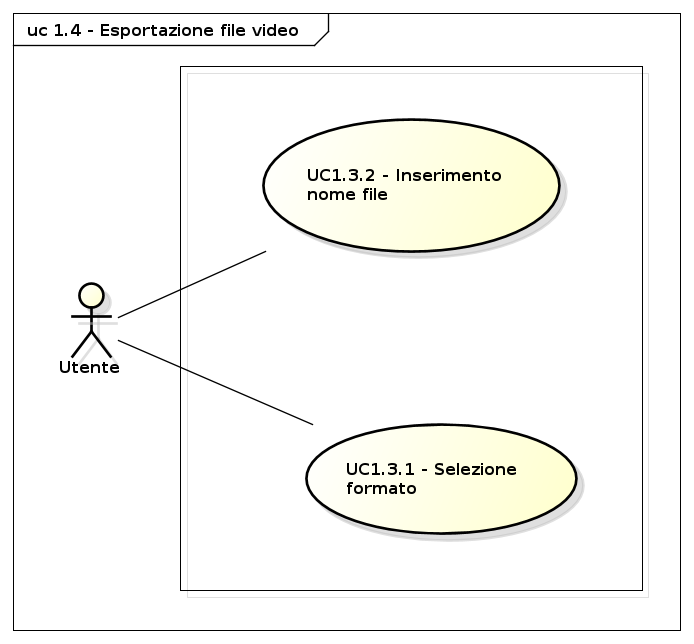
\includegraphics[scale=0.5]{immagini/uc1_4_esportazione_video.png}
\captionsetup{labelfont=bf}
\caption{Caso d'uso UC1.4}
\end{figure}
\newpage

\subsection{Caso d'uso UC1.5: Salvataggio file}
\label{sec:UC1.5}

\begin{itemize}
\item \textbf{Attori}: utente, sistema;
\item \textbf{Scopo e descrizione}: l'utente può salvare le modifiche apportate a uno sceneggiato; il sistema provvede al salvataggio effettivo reperendo la cartella di destinazione impostata di default;
\item \textbf{Precondizione}: il sistema è pronto a effettuare il salvataggio;
\item \textbf{Flusso principale degli eventi}:
\begin{enumerate}
\item Il sistema reperisce la cartella di default (UC1.5.1);
\item Il sistema effettua il salvataggio (UC1.5.2). 
\end{enumerate} 
\item \textbf{Scenari alternativi}: il sistema avverte l'utente in caso il salvataggio non andasse a buon fine (ad esempio a causa di mancanza di memoria disponibile) (UC1.5.3);
\item \textbf{Postcondizione}: il salvataggio viene effettuato correttamente. 
\end{itemize}
\begin{figure}[htbp]
\centering
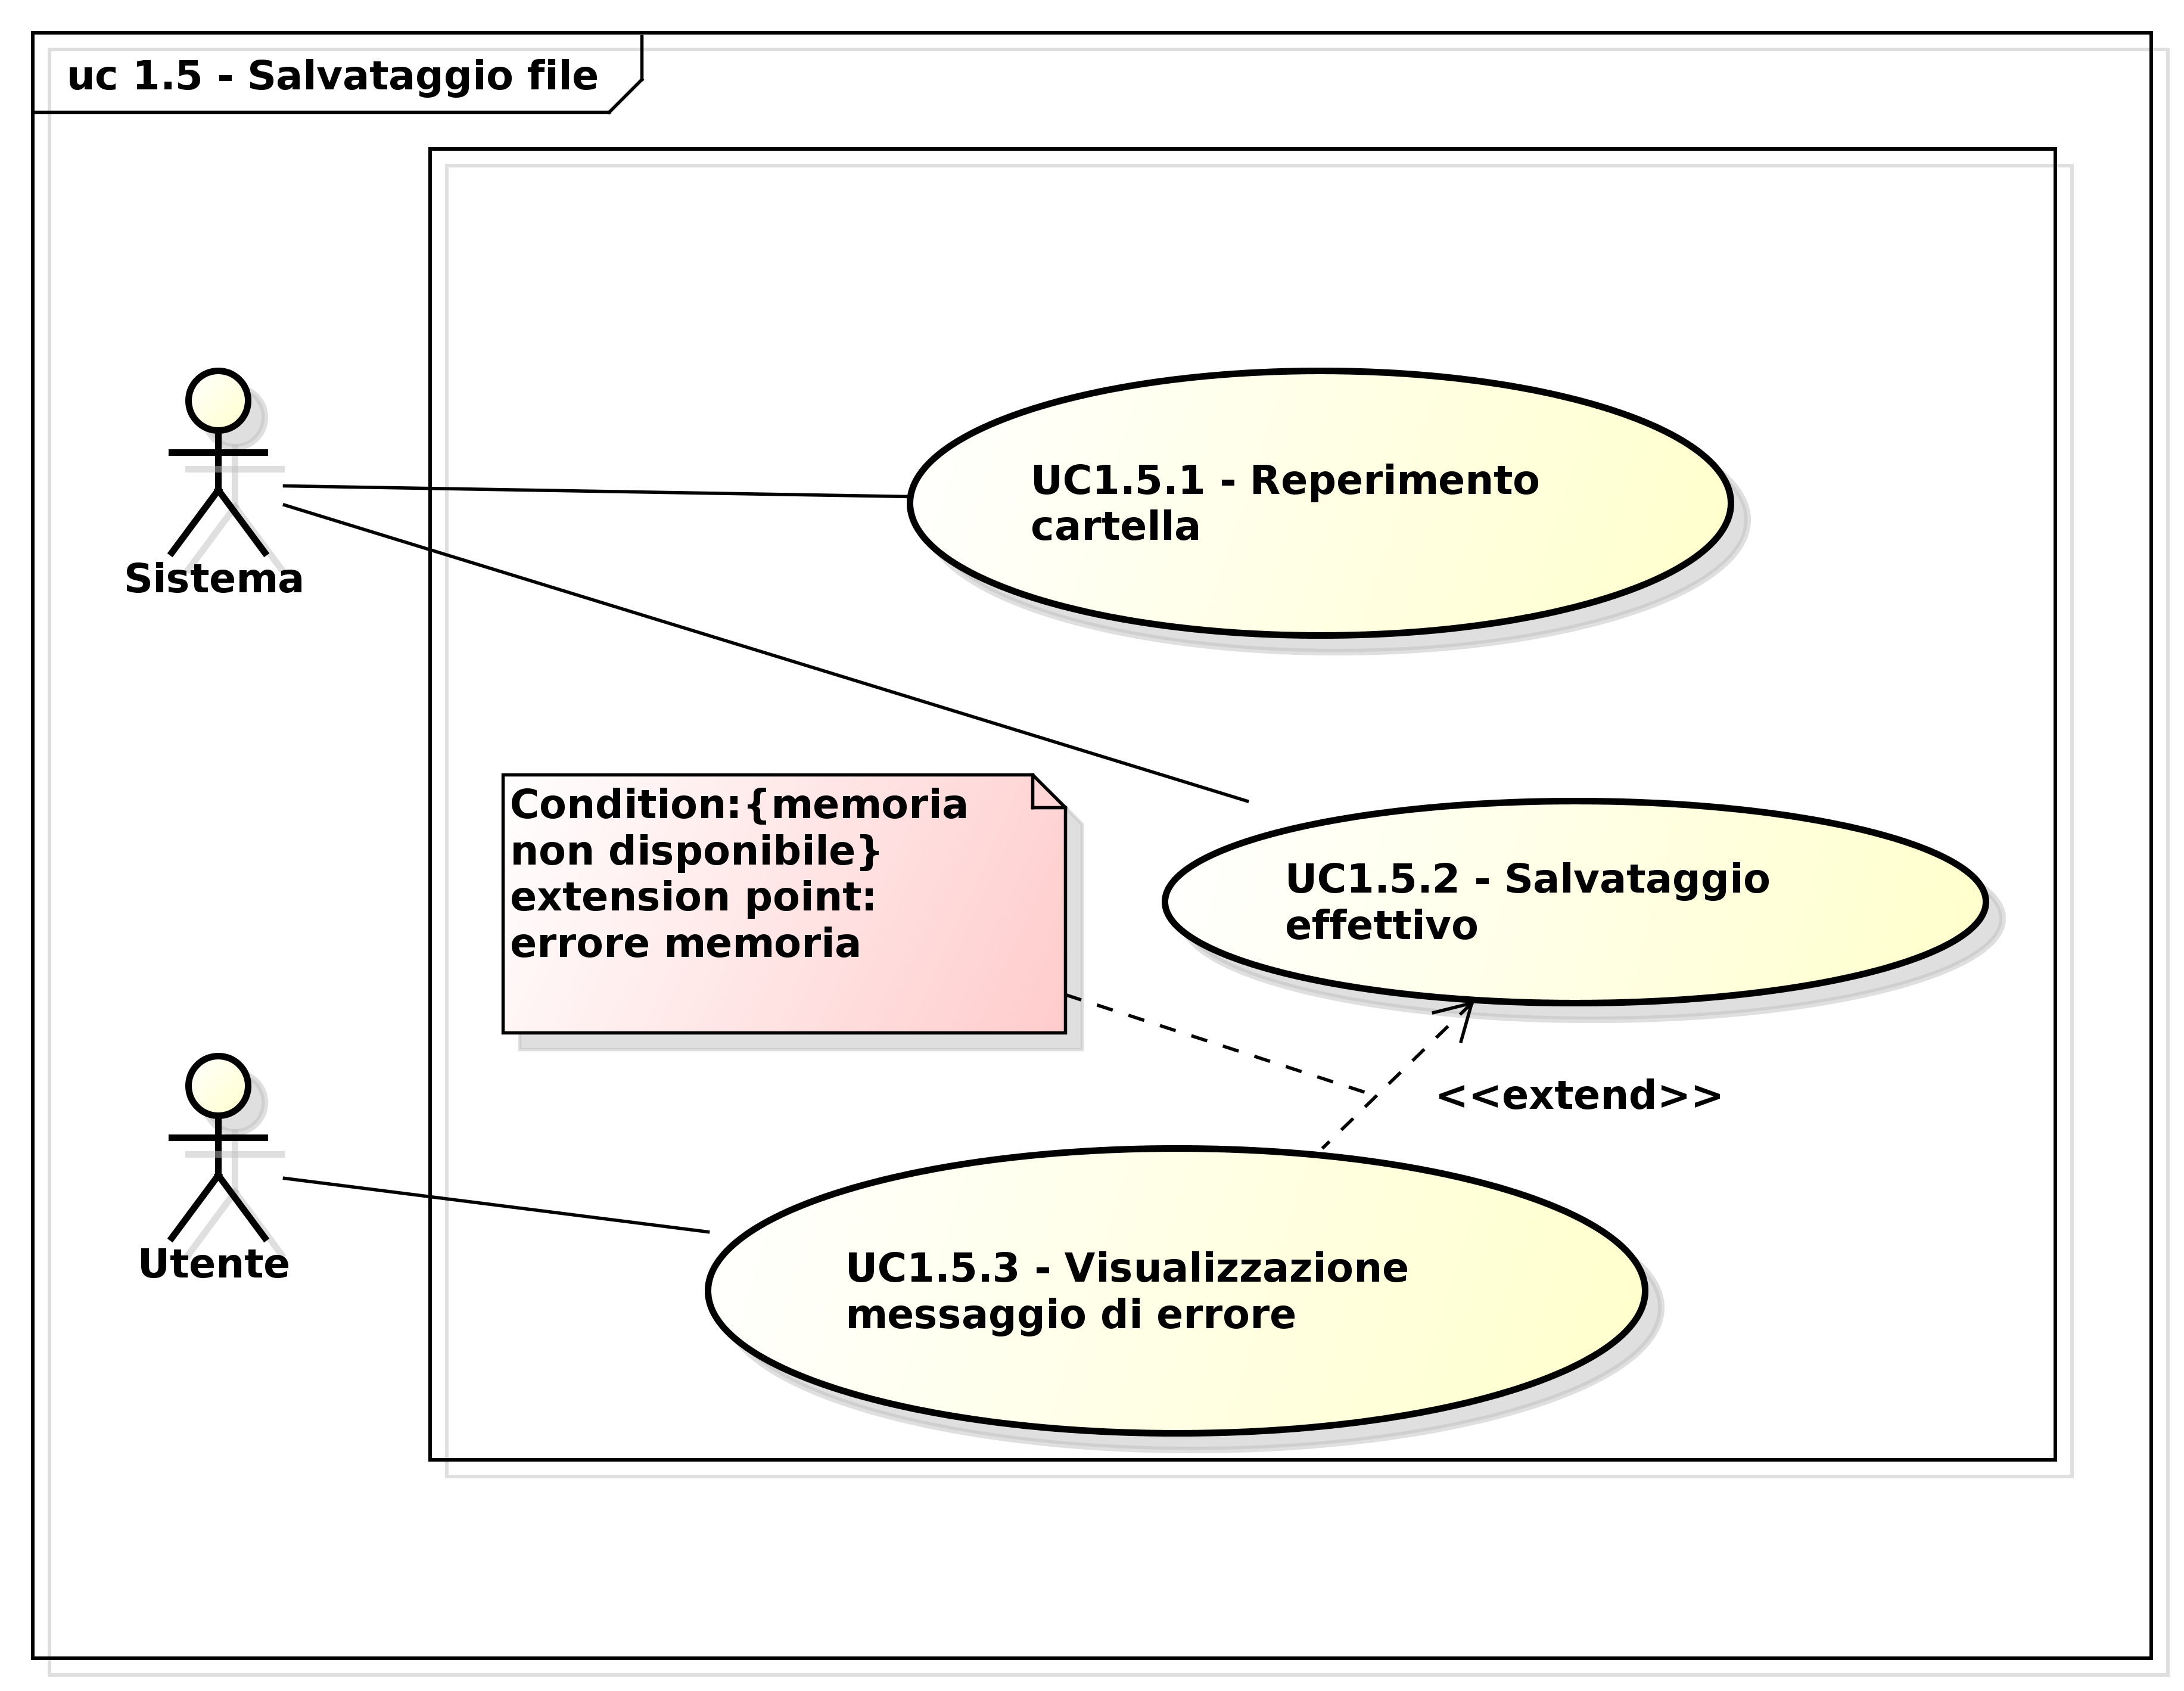
\includegraphics[scale=0.5]{immagini/uc1_5_salvataggio_file.png}
\captionsetup{labelfont=bf}
\caption{Caso d'uso UC1.5}
\end{figure}
\newpage

\subsection{Caso d'uso UC1.7: Apertura file}
\label{sec:UC1.7}

\begin{itemize}
\item \textbf{Attori}: utente;
\item \textbf{Scopo e descrizione}: navigando fra i \textit{file} di sistema, l'utente può selezionare un \textit{file} specifico da aprire;
\item \textbf{Precondizione}: il programma è avviato e viene richiesto il caricamento di un \textit{file};
\item \textbf{Flusso principale degli eventi}:
\begin{enumerate}
\item L'utente naviga fra i \textit{file} di sistema (UC1.7.0.1);
\item L'utente seleziona il \textit{file} da aprire (UC.1.7.0.2);
\item L'utente conferma l'apertura del \textit{file} selezionato (UC1.7.0.3).
\end{enumerate}
\item \textbf{Scenari alternativi}: il \textit{file} selezionato non è conforme alla tipologia di \textit{file} richiesto: in questo caso viene visualizzato un opportuno messaggio d'errore;
\item \textbf{Postcondizione}: il \textit{file} viene aperto correttamente.
\end{itemize}
\begin{figure}[htbp]
\centering
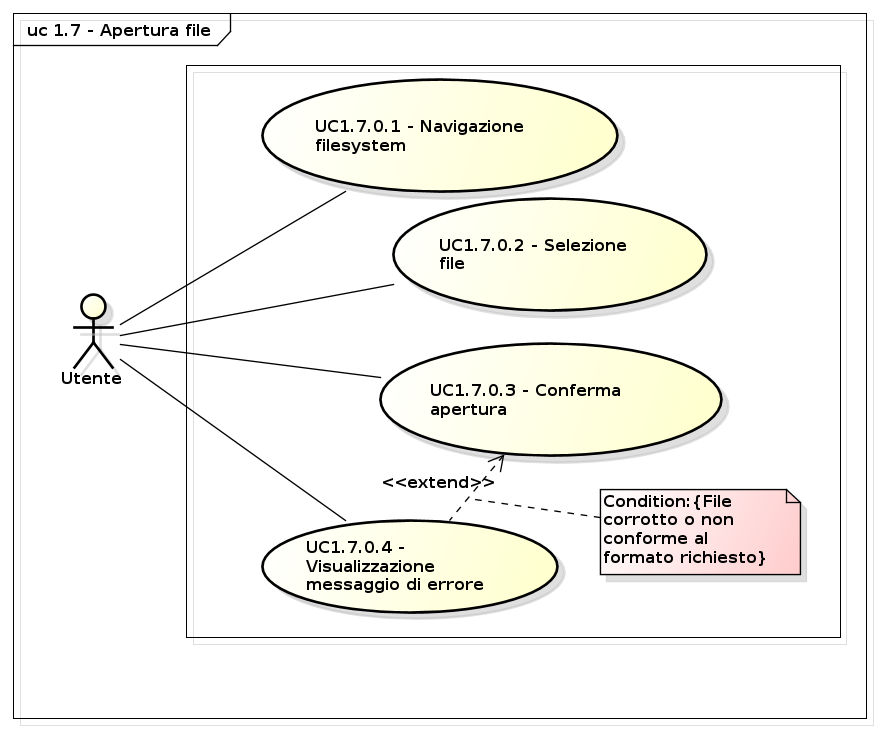
\includegraphics[scale=0.5]{immagini/uc1_7_apertura_file.png}
\captionsetup{labelfont=bf}
\caption{Caso d'uso UC1.7}
\end{figure}
\newpage

\subsection{Caso d'uso UC1.8: Modifica sceneggiato}
\label{sec:UC1.8}

\begin{itemize}
\item \textbf{Attori}: utente;
\item \textbf{Scopo e descrizione}: l'utente può aprire uno sceneggiato già creato e modificarlo;
\item \textbf{Precondizione}: esiste almeno uno sceneggiato creato in precedenza;
\item \textbf{Flusso principale degli eventi}:
\begin{enumerate}
\item L'utente apre lo sceneggiato da modificare (UC1.7.2);
\item L'utente può modificare un capitolo dello sceneggiato (UC1.8.1);
\item L'utente può avere un'anteprima dello sceneggiato appena modificato (UC1.8.2);
\end{enumerate}
\item \textbf{Postcondizione}: lo sceneggiato viene modificato correttamente.
\end{itemize}
\begin{figure}[htbp]
\centering
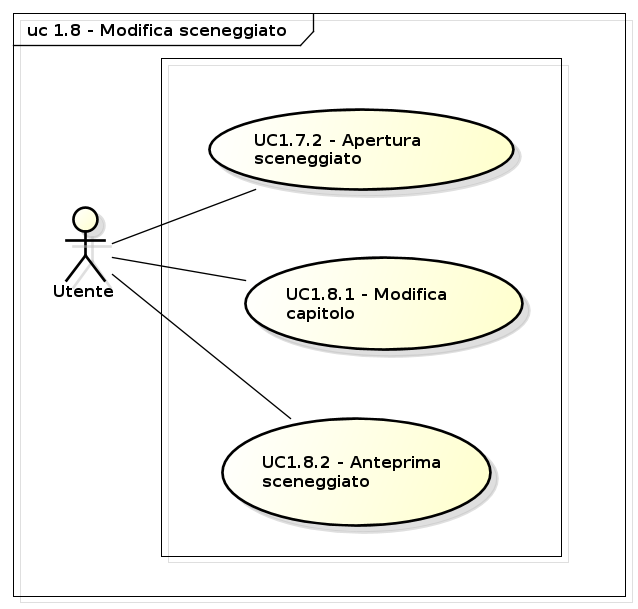
\includegraphics[scale=0.5]{immagini/uc1_8_modifica_sceneggiato.png}
\captionsetup{labelfont=bf}
\caption{Caso d'uso UC1.8}
\end{figure}
\newpage

\subsection{Caso d'uso UC1.8.1: Modifica capitolo}
\label{sec:UC1.8.1}

\begin{itemize}
\item \textbf{Attori}: utente;
\item \textbf{Scopo e descrizione}: l'utente può modificare un capitolo di uno sceneggiato già creato; nello specifico può modificarne lo sfondo, una o più battute, il titolo e i suoni di arricchimento;
\item \textbf{Precondizione}: nello sceneggiato è stato creato almeno un capitolo;
\item \textbf{Flusso principale degli eventi}:
\begin{enumerate}
\item L'utente seleziona il capitolo da modificare (UC1.8.1.1);
\item L'utente può vedere un'anteprima del capitolo (UC1.8.1.2);
\item L'utente può modificarne il titolo (UC1.8.1.4);
\item L'utente può modificarne lo sfondo (UC1.8.1.3);
\item L'utente può modificarne una battuta (UC1.1.2.4);
\item L'utente può cancellare una battuta del capitolo (UC1.1.2.5);
\item L'utente può inserire un nuovo suono di arricchimento o cancellarne uno inserito in precedenza (UC1.1.2.6, UC1.8.1.5).
\end{enumerate}
\item \textbf{Postcondizione}: il capitolo viene modificato correttamente.
\end{itemize}
\begin{figure}[htbp]
\centering
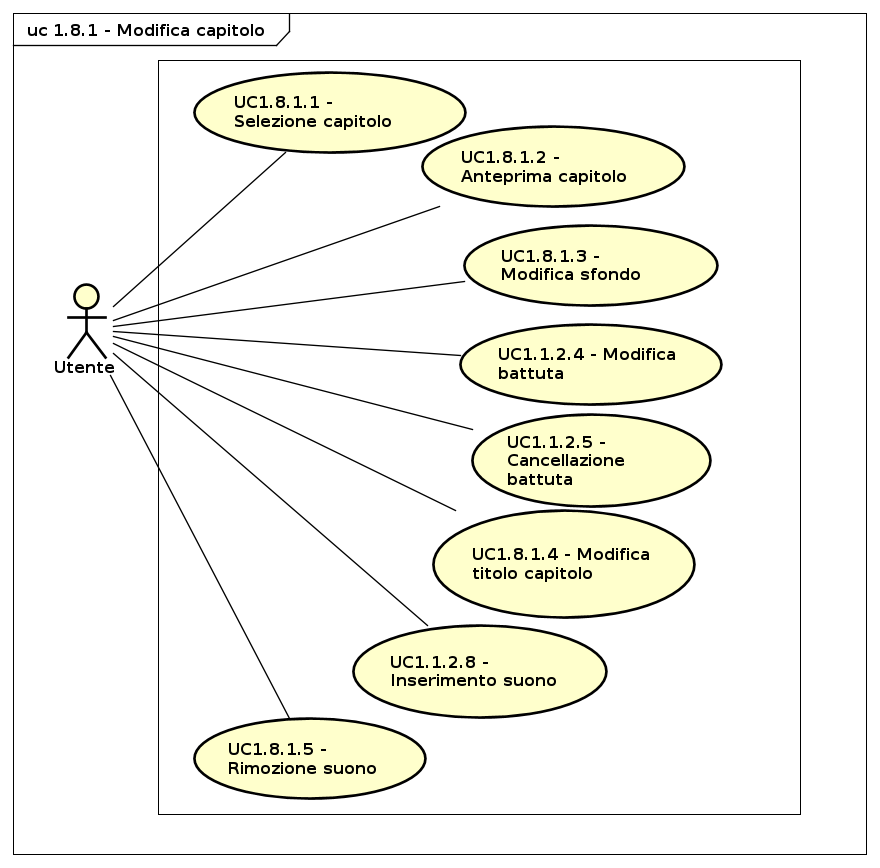
\includegraphics[scale=0.5]{immagini/uc1_8_1_modifica_capitolo.png}
\captionsetup{labelfont=bf}
\caption{Caso d'uso UC1.8.1}
\end{figure}
\newpage

\subsection{Caso d'uso UC2: Configurazione alto livello}
\label{sec:UC2}

\begin{itemize}
\item \textbf{Attori}: utente;
\item \textbf{Scopo e descrizione}: l'utente può creare nuovi \textit{preset}\G, modificando parametri ed effetti.  Inoltre può selezionare una nuova voce da impostare per il sistema e campionare la propria;
\item \textbf{Precondizione}: l'applicazione è stata avviata correttamente;
\item \textbf{Flusso principale degli eventi}:
\begin{enumerate}
\item L'utente può creare un nuovo \textit{preset} o modificarne uno già creato (UC2.1, UC2.5);
\item L'utente può testare il \textit{preset} creato (UC2.4); 
\item L'utente può selezionare una voce per il sistema (UC2.2);
\item L'utente può campionare la sua voce (UC2.3).
\end{enumerate}
\item \textbf{Postcondizione}: l'applicazione agisce secondo le direttive dell'utente.
\end{itemize}
\begin{figure}[htbp]
\centering
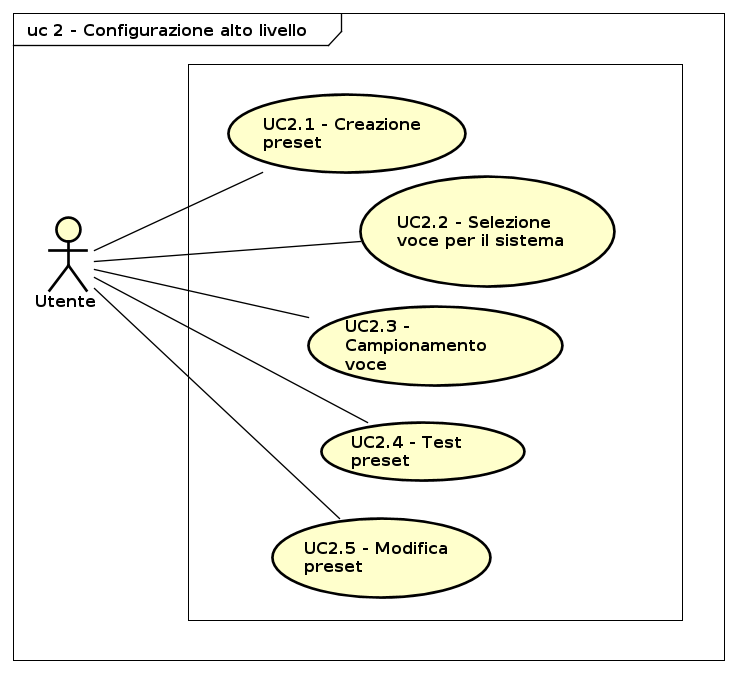
\includegraphics[scale=0.5]{immagini/uc2_configurazione_alto_livello.png}
\captionsetup{labelfont=bf}
\caption{Caso d'uso UC2}
\end{figure}
\newpage


\subsection{Caso d'uso UC2.1: Creazione preset}
\label{sec:UC2.1}

\begin{itemize}
\item \textbf{Attori}: utente, modulo di sistema;
\item \textbf{Scopo e descrizione}: dopo che il modulo di sistema ha reperito gli effetti disponibili, l'utente può navigare tra questi, selezionarli e associarli a voci; l'utente può infine salvare i cambiamenti apportati;
\item \textbf{Precondizione}: il sistema ha reperito gli effetti disponibili;
\item \textbf{Flusso principale degli eventi}:
\begin{enumerate}
\item Il modulo reperisce gli effetti (UC3.2);
\item L'utente può navigare tra gli effetti disponibili (UC2.1.1);
\item L'utente può settare dei parametri (UC2.1.2);
\item L'utente può salvare il \textit{preset}\G\ creato (UC2.1.3).
\end{enumerate}
\item \textbf{Postcondizione}: è stato salvato un \textit{preset} creato dall'utente.
\end{itemize}
\begin{figure}[htbp]
\centering
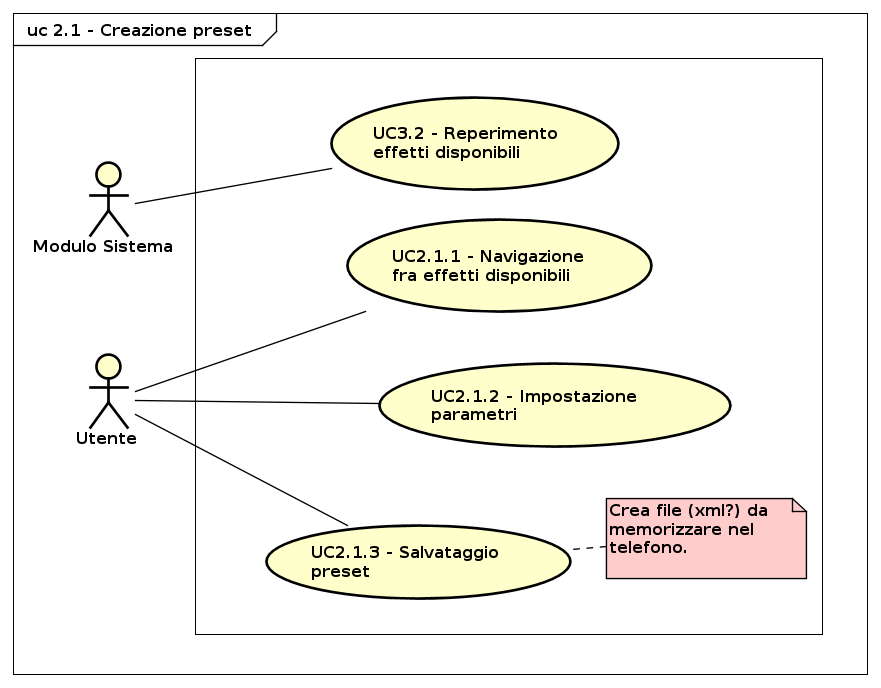
\includegraphics[scale=0.5]{immagini/uc2_1_creazione_preset.png}
\captionsetup{labelfont=bf}
\caption{Caso d'uso UC2.1}
\end{figure}
\newpage

\subsection{Caso d'uso UC2.2: Selezione voce per il sistema}
\label{sec:UC2.2}

\begin{itemize}
\item \textbf{Attori}: utente;
\item \textbf{Scopo e descrizione}: l'utente può impostare una delle voci disponibili come voce di default per il sistema, oppure può scegliere di crearne una nuova;
\item \textbf{Precondizione}: esistono delle voci disponibili;
\item \textbf{Postcondizione}: la voce è stata impostata correttamente.
\end{itemize}
\begin{figure}[htbp]
\centering
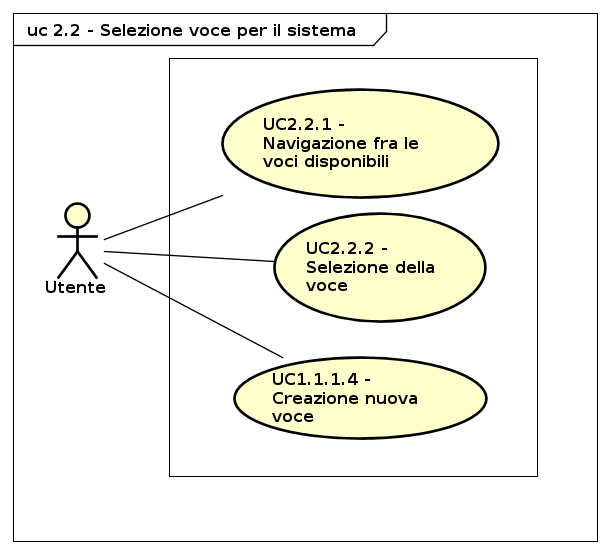
\includegraphics[scale=0.5]{immagini/uc2_2_selezione_voce_sistema.png}
\captionsetup{labelfont=bf}
\caption{Caso d'uso UC2.2}
\end{figure}
\newpage

\subsection{Caso d'uso UC2.3: Campionamento voce}
\label{sec:UC2.3}

\begin{itemize}
\item \textbf{Attori}: utente, applicazione;
\item \textbf{Scopo e descrizione}: l'utente può campionare la sua voce  eseguendo una procedura che prevede la lettura e la registrazione di frasi, che verranno inviate in formato audio dall'applicazione al server di \AZIENDA;
\item \textbf{Precondizione}: il sistema è pronto per il campionamento;
\item \textbf{Flusso principale degli eventi}:
\begin{enumerate}
\item L'utente effettua la login\G\ al servizio web di MIVOQ (UC2.3.4);
\item L'utente visualizza le frasi da leggere (UC2.3.1);
\item Viene registrata la lettura delle frasi (UC2.3.2);
\item L'applicazione invia la registrazione al server per il campionamento, per poi ricominciare dal punto 1. mostrando all'utente una nuova frase da leggere (UC2.3.3);
\item L'utente può decidere di terminare la sessione di campionamento, per continuare in un secondo momento.
\end{enumerate}
\item \textbf{Postcondizione}: il campionamento è andato a buon fine.
\end{itemize}
\begin{figure}[htbp]
\centering
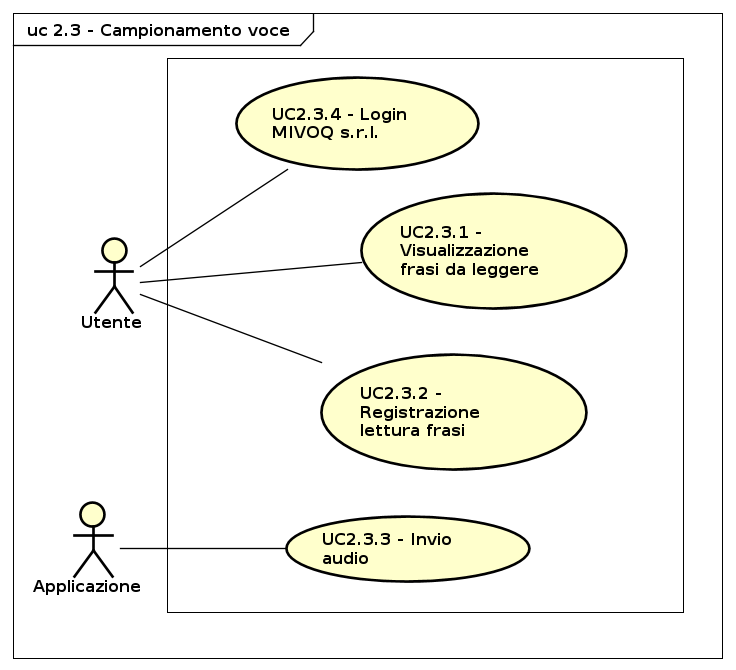
\includegraphics[scale=0.5]{immagini/uc2_3_campionamento_voce.png}
\captionsetup{labelfont=bf}
\caption{Caso d'uso UC2.3}
\end{figure}
\newpage

\subsection{Caso d'uso UC2.4: Test preset}
\label{sec:UC2.4}

\begin{itemize}
\item \textbf{Attori}: utente;
\item \textbf{Scopo e descrizione}: l'utente può ascoltare il \textit{preset}\G;
\item \textbf{Precondizione}: il \textit{preset} è stato creato correttamente;
\item \textbf{Postcondizione}: viene riprodotto l'audio di un testo di prova con il \textit{preset} associato.
\end{itemize}
\begin{figure}[htbp]
\centering
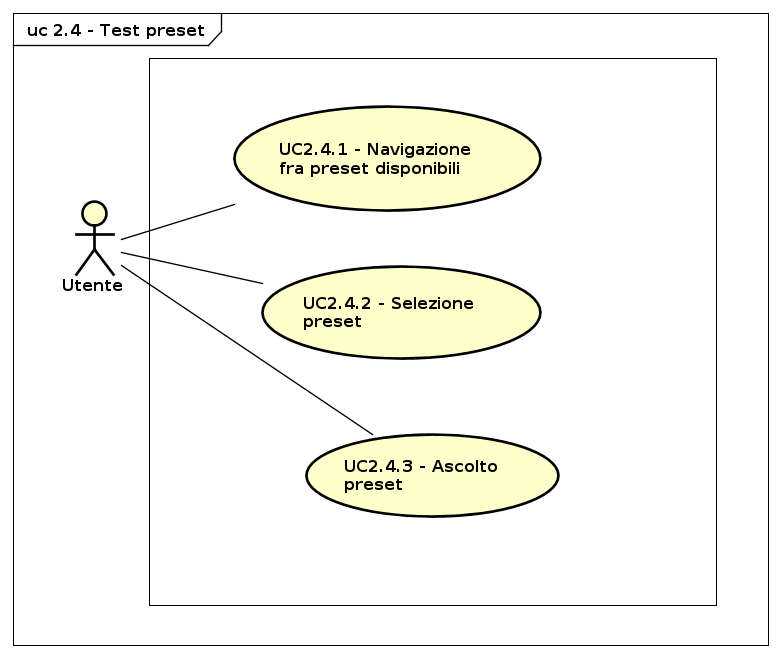
\includegraphics[scale=0.5]{immagini/uc2_4_test_preset.png}
\captionsetup{labelfont=bf}
\caption{Caso d'uso UC2.4}
\end{figure}
\newpage

\subsection{Caso d'uso UC2.5: Modifica preset}
\label{sec:UC2.5}

\begin{itemize}
\item \textbf{Attori}: utente;
\item \textbf{Scopo e descrizione}: l'utente può aprire un \textit{preset}\G\ già creato e modificarlo;
\item \textbf{Precondizione}: viene selezionato un \textit{preset} correttamente creato; 
\item \textbf{Flusso principale degli eventi}:
\begin{enumerate}
\item L'utente seleziona il \textit{preset} da modificare (UC2.5.1);
\item L'utente modifica i parametri del \textit{preset} (UC2.5.2);
\item L'utente salva le modifiche apportate (UC2.5.3).
\end{enumerate}
\item \textbf{Postcondizione}: il \textit{preset} viene modificato e salvato correttamente.
\end{itemize}
\begin{figure}[htbp]
\centering
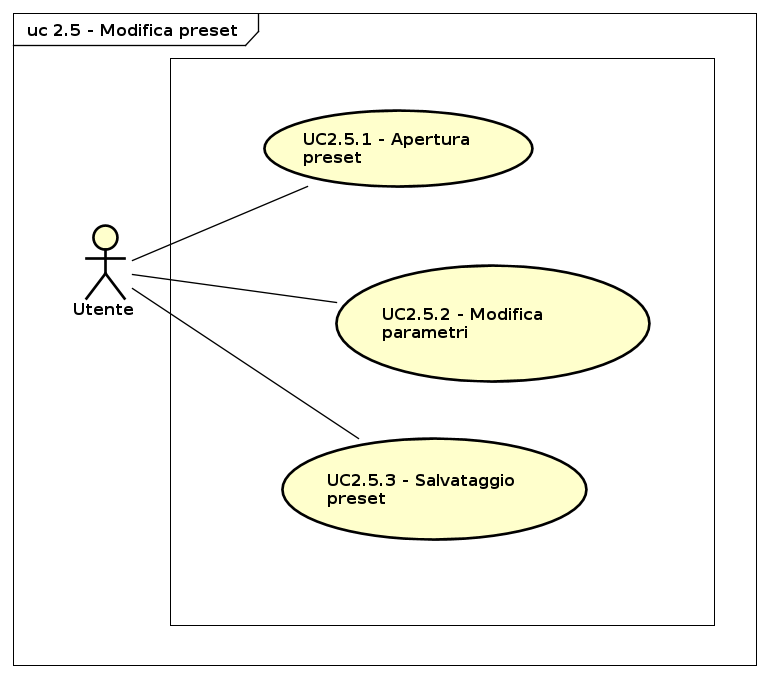
\includegraphics[scale=0.5]{immagini/uc2_5_modifica_preset.png}
\captionsetup{labelfont=bf}
\caption{Caso d'uso UC2.5}
\end{figure}
\newpage

\subsection{Caso d'uso UC3: Modulo di sistema alto livello}
\label{sec:UC3}

\begin{itemize}
\item \textbf{Attori}: modulo di sistema;
\item \textbf{Scopo e descrizione}: il modulo di sistema può reperire gli effetti e le voci disponibili comunicando con il server di \AZIENDA. Ogni comunicazione con il server avviene attraverso questa componente;
\item \textbf{Precondizione}: il modulo è pronto ad operare;
\item \textbf{Flusso principale degli eventi}:
\begin{enumerate}
\item Il modulo di sistema reperisce le voci disponibili (UC3.1);
\item Il modulo di sistema reperisce gli effetti disponibili (UC3.2);
\item Il modulo di sistema reperisce i \textit{file} audio (UC3.4);
\item Il modulo di sistema seleziona il \textit{preset}\G\ per il sistema (UC3.5);
\item Il modulo di sistema converte le battute in SSML\G\ (UC3.6);
\end{enumerate}
\item \textbf{Postcondizione}: il modulo svolge quanto richiesto;
\item \textbf{Generalizzazione}: il reperimento delle voci, degli effetti e la ricezione dell'audio sono azioni specifiche, che prevedono la comunicazione con il server di \AZIENDA.
\end{itemize}
\begin{figure}[htbp]
\centering
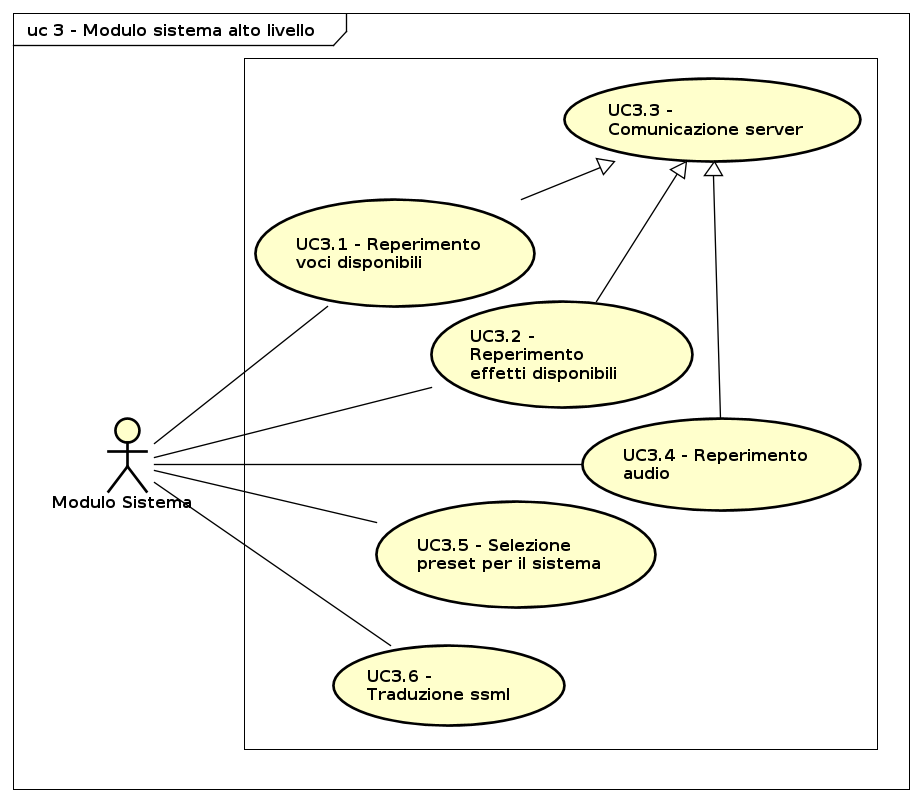
\includegraphics[scale=0.5]{immagini/uc3_modulo_sistema_alto_livello.png}
\captionsetup{labelfont=bf}
\caption{Caso d'uso UC3}
\end{figure}
\newpage

\subsection{Caso d'uso UC3.3: Comunicazione server}
\label{sec:UC3.3}

\begin{itemize}
\item \textbf{Attori}: modulo di sistema, utente;
\item \textbf{Scopo e descrizione}: il modulo di sistema crea una richiesta HTTP\G, la invia al server di \AZIENDA\ e attende una risposta da quest'ultimo; in caso di connessione alla rete assente viene mostrato all'utente un messaggio d'errore;
\item \textbf{Precondizione}: il modulo è pronto a comunicare con il server;
\item \textbf{Flusso principale degli eventi}:
\begin{enumerate}
\item Il modulo crea una richiesta HTTP (UC3.3.1);
\item Il modulo invia la richiesta HTTP creata (UC3.3.2);
\item Il modulo riceve una risposta dal server (UC3.3.3).
\end{enumerate}
\item \textbf{Scenari alternativi}: nel caso in cui non fosse possibile comunicare con il server a causa di connessione alla rete assente, il sistema avverte l'utente con un messaggio d'errore;  
\item \textbf{Postcondizione}: la comunicazione va a buon fine.
\end{itemize}
\begin{figure}[htbp]
\centering
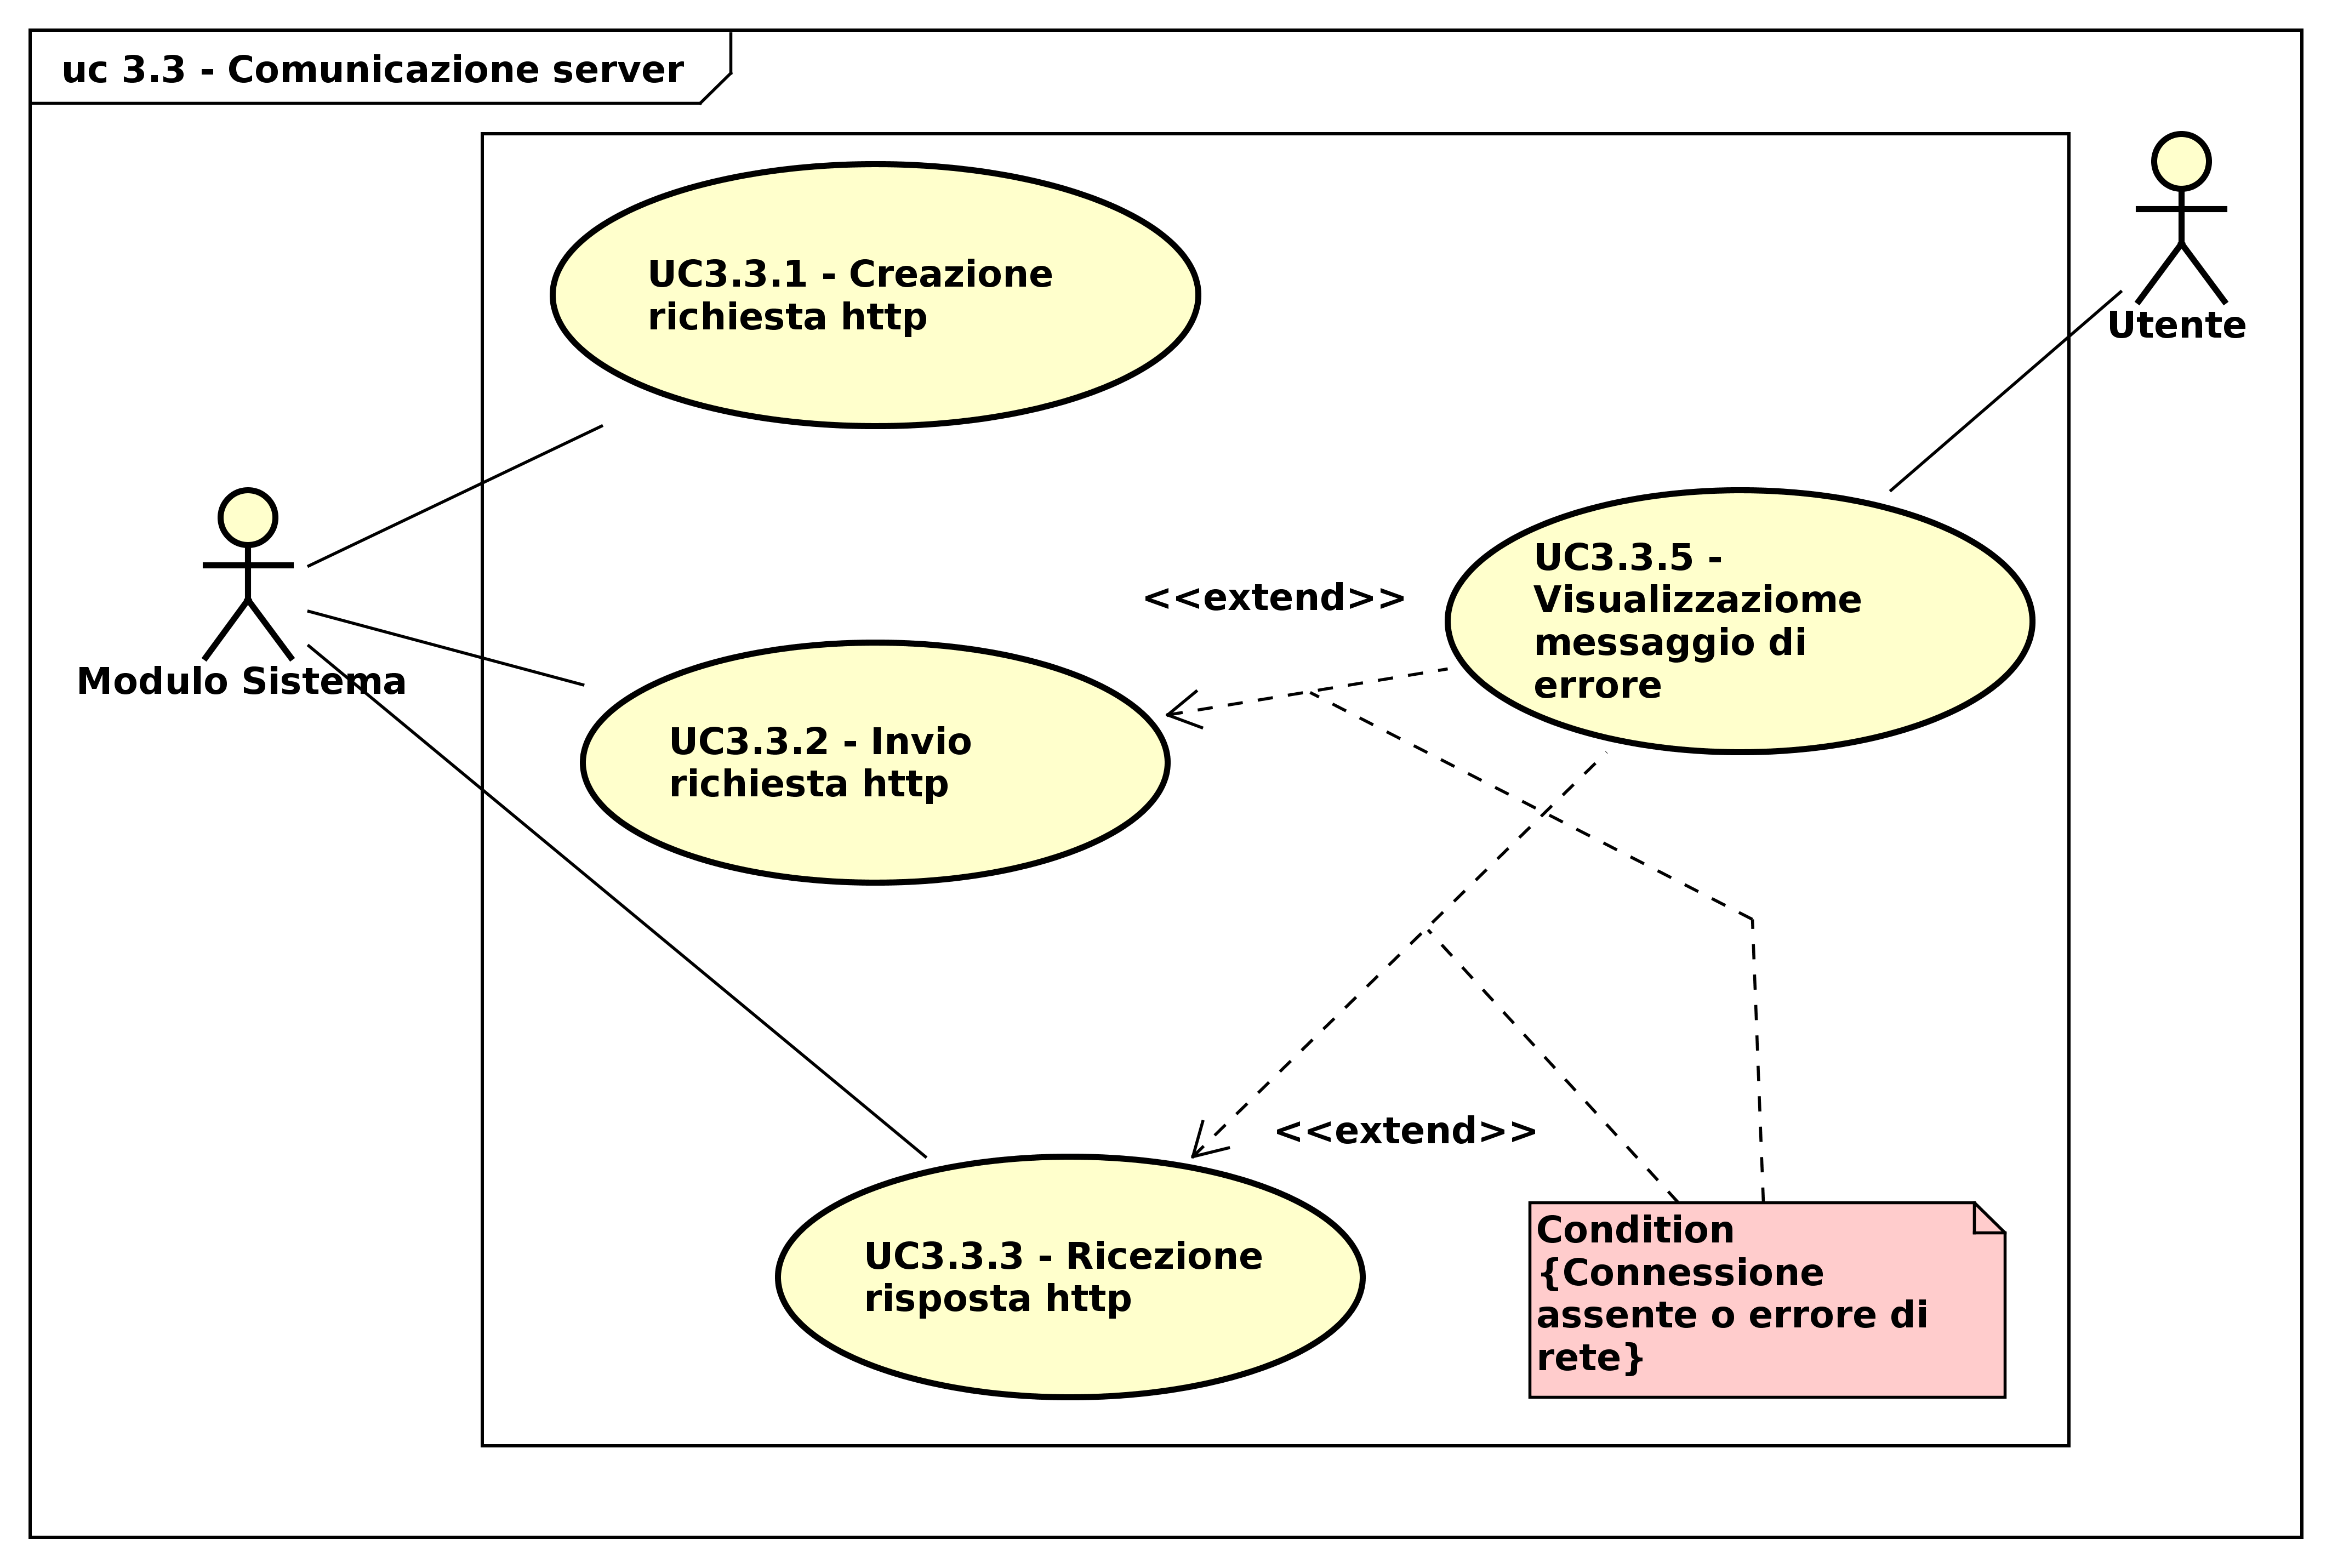
\includegraphics[scale=0.5]{immagini/uc3_3_comunicazione_server.png}
\captionsetup{labelfont=bf}
\caption{Caso d'uso UC3.3}
\end{figure}
\newpage

%\subsection{Caso d'uso UC3.5: Selezione preset}
%\label{sec:UC3.5}
%\begin{itemize}
%\item \textbf{Attori}: modulo di sistema;
%\item \textbf{Scopo e descrizione}: il modulo di sistema salva il \textit{preset}\G\ selezionato su un %\textit{file} di configurazione;
%\item \textbf{Precondizione}: esiste almeno un \textit{preset} disponibile;
%\item \textbf{Postcondizione}: il \textit{preset} è stato selezionato e impostato.
%\end{itemize}
%\begin{figure}[htbp]
%\centering
%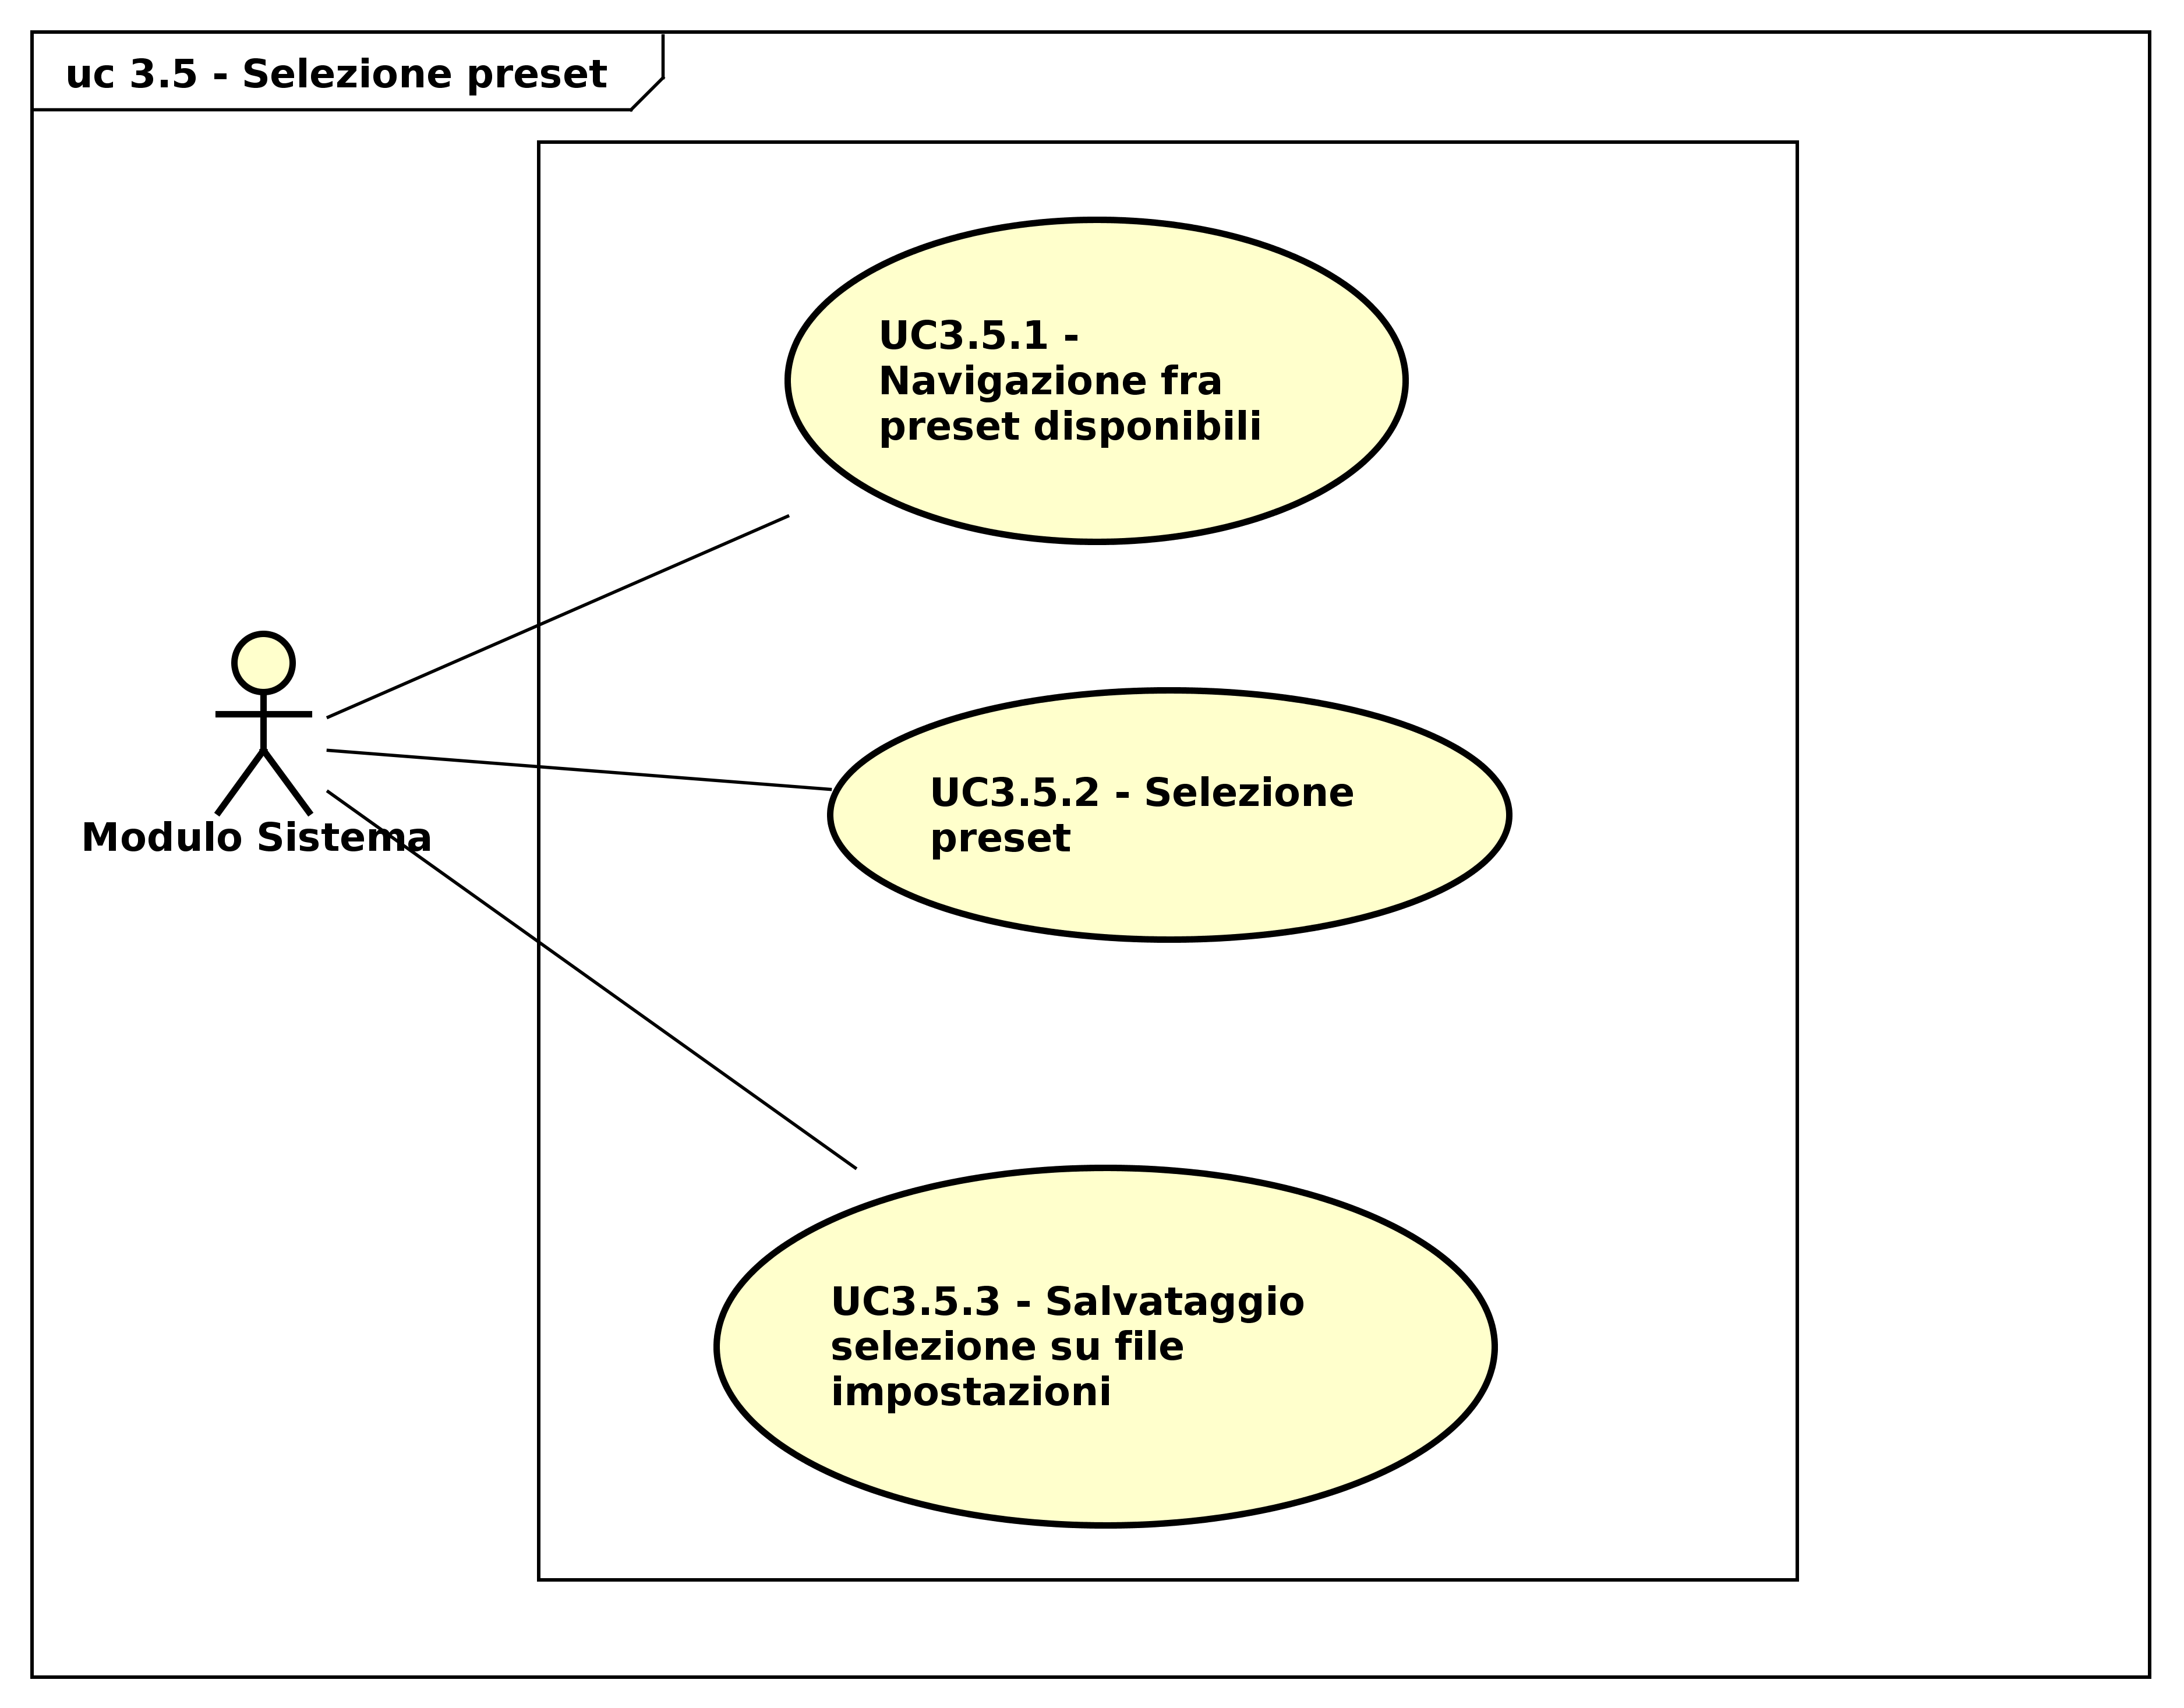
\includegraphics[scale=0.5]{immagini/uc3_5_selezione_preset.png}
%\captionsetup{labelfont=bf}
%\caption{Caso d'uso UC3.5}
%\end{figure}
%\newpage

\subsection{Caso d'uso UC3.6: Traduzione SSML}
\label{sec:UC3.6}

\begin{itemize}
\item \textbf{Attori}: modulo di sistema;
\item \textbf{Scopo e descrizione}: il modulo di sistema converte il testo delle battute inserite dall'utente nello sceneggiato in SSML\G;
\item \textbf{Precondizione}: il modulo ha ricevuto correttamente il testo inserito dall'utente;
\item \textbf{Flusso principale degli eventi}:
\begin{enumerate}
\item Il modulo esegue l'\textit{encoding}\G\ e l'\textit{escaping}\G\ del testo (UC3.6.1);
\item Il modulo crea i \textit{tag}\G\ conformi al linguaggio SSML (UC3.6.2);
\item Il modulo inserisce i parametri e gli attributi nei \textit{tag} (UC3.6.3).
\end{enumerate}
\item \textbf{Postcondizione}: il testo è stato convertito correttamente seguendo le regole del linguaggio SSML.
\end{itemize}
\begin{figure}[htbp]
\centering
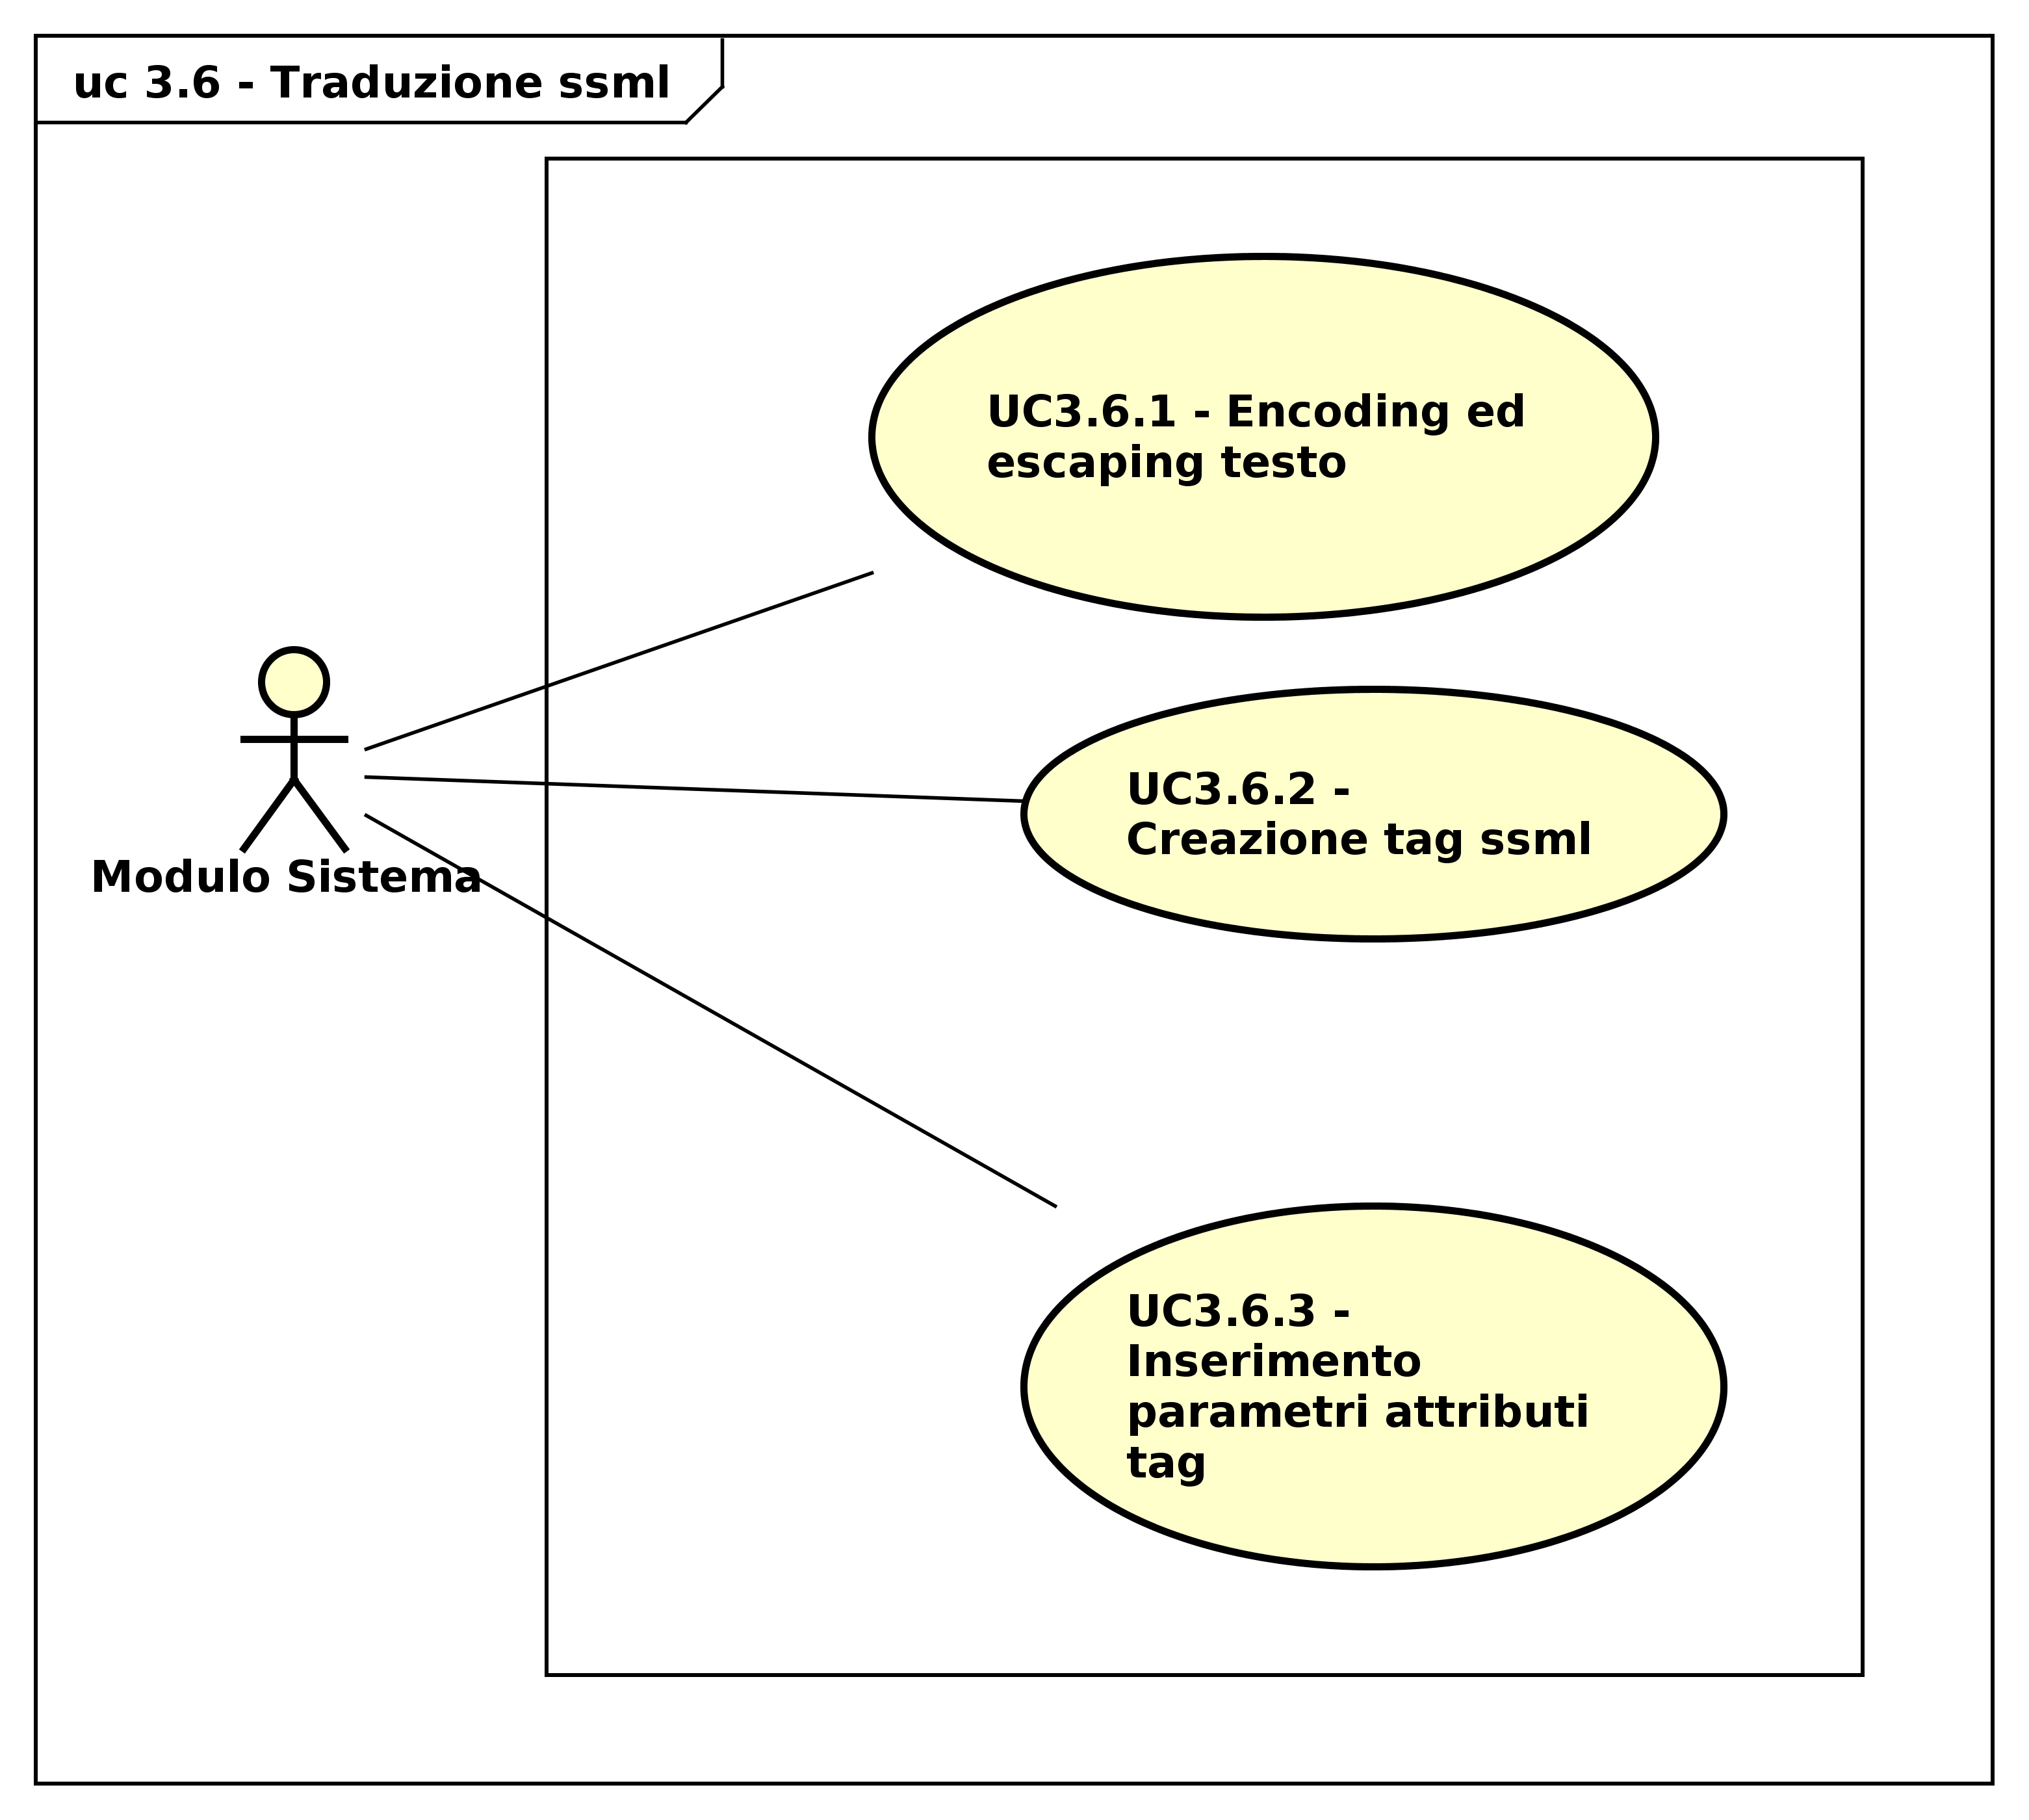
\includegraphics[scale=0.5]{immagini/uc3_6_traduzione_ssml.png}
\captionsetup{labelfont=bf}
\caption{Caso d'uso UC3.5}
\end{figure}
\newpage